\documentclass[12 pt, oneside]{book}
\usepackage{graphicx, fancyhdr, amsmath, times,  enumerate,geometry,makeidx,setspace,nomencl,eso-pic,xcolor,lipsum,calc,pst-node,tikz,fancybox,background,caption,subcaption,amsfonts,ragged2e}



\usetikzlibrary{calc}
\SetBgScale{1}
\SetBgAngle{0}
\SetBgColor{brown}
\SetBgOpacity{1}
%%
\geometry{verbose,a4paper,tmargin=1in,bmargin=1in,lmargin=1.5 in,rmargin=.9 in}
%%%%%%%%%%%%%%%%%%%%%%%%%%%%%%%

\makeindex

%%
\usepackage[final]{pdfpages}
%%
%\setlength{\oddsidemargin}{2 cm}
%%
\newcommand{\VAtitle}[1]%
{\def\vtitle{#1}}%
\newcommand{\VAauthor}[1]%
{\def\vauthor{#1}}%
\newcommand{\VAauthora}[1]%
{\def\vauthora{#1}}%
\newcommand{\VAauthorb}[1]%
{\def\vauthorb{#1}}%
\newcommand{\VAauthorc}[1]%
{\def\vauthorc{#1}}%
\newcommand{\VAauthord}[1]%
{\def\vauthord{#1}}%
\newcommand{\VAauthore}[1]%
{\def\vauthore{#1}}%
\newcommand{\VAadmissionyear}[1]%
{\def\vadmissionyear{#1}}%
\newcommand{\VAacademicyear}[1]%
{\def\vacademicyear{#1}}%
\newcommand{\VAregisternumber}[1]%
{\def\vregisternumber{#1}}%
\newcommand{\VAprincipal}[1]%
{\def\vprincipal{#1}}%
\newcommand{\VAguide}[1]%
{\def\vguide{#1}}%
\newcommand{\VAguidedg}[1]%
{\def\vguidedg{#1}}%
\newcommand{\VAhod}[1]%
{\def\vhod{#1}}%
\newcommand{\VAmonth}[1]%
{\def\vmonth{#1}}%
\newcommand{\VAdept}[1]%
{\def\vdept{#1}}%
\newcommand{\VAdate}[1]%
{\def\vdate{#1}}%
\newcommand{\VAclass}[1]%
{\def\vclass{#1}}%
\newcommand{\VApaper}[1]%
{\def\vpaper{#1}}%
%%
%%
%\renewcommand\bibname{References}




\SetBgContents{}

\VApaper{FINAL YEAR PROJECT REPORT}

\usepackage{tabularx}
\usepackage{titlesec}
\titleformat{\chapter}[display]
{\normalfont\huge\bfseries\centering}{\chaptertitlename\ \thechapter}{2pt}{\Huge}

\begin{document}
%%%%%%%%%%%%%%%%%%%%%%%%%%%%%%%%%%%%
%%%%%%%%%%%%%%%%%%%%%%%%%%%%%%%%%%%%
%	Edit from Below . . . 
%   In the next line, replace "ReportTitle" by 
%   the title of PROJECT
%
\VAtitle{RESUME SCREENING}
%
%
%   In the next line, replace "Student" by your name. 
%   Write full name without, Mr. or Ms.
%

\VAauthora{AATHIRA P R}
\VAauthorb{ABHIRAMI ANANTHAKUMAR}
\VAauthorc{AMAL CEZNA}
\VAauthord{JEWELNA T J}
%
%
%
\VAauthor{STUDENT NAME}
\VAadmissionyear{2019}%
%
\VAacademicyear{2022-2023}%
%
%   University Examination Register Number.
%

% 
%
%   the full name of your principal
%
\VAprincipal{Dr.Vijayan P}
%   In the next line, replace "HoD" by the full name of Head of Department with Mr. or Ms. or Dr. or Prof.
%
\VAhod{Dr.Suresan Pareth}
%
%  the full name of your guide or supervisor 
\VAguide{Mrs.Jyothi P Joy}% 
\VAguidedg{Asst. Prof.,} % Give your Guides Designation Asst. Prof., Asso. Prof.
%   Enter the Sem End month like "December"
%   Type Month and Year
\VAmonth{June 2023}%
\VAdept{Computer Science and Engineering}%
\VAclass{Eighth Semester B.Tech}%
%%%%%%%%%%%%%%%%%%%%%%%%%%%%%%%%%%%%%
%%%%%%%%%%%%%%%%%%%%%%%%%%%%%%%%%%%%%
\fancypagestyle{plain}{%
\fancyhf{} % clear all header and footer fields
\fancyhead[L]{{\scriptsize \vtitle}}
\fancyhead[R]{\footnotesize Final year project report}
%\fancyfoot[C]{\bfseries \thepage} 
\fancyfoot[L]{{\footnotesize Department of  \vdept\ }}
\fancyfoot[R]{\footnotesize Thejus Engg college, Vellarakkad}
\fancyfoot[C]{\footnotesize \bf \thepage}%
\SetBgContents{

\begin{tikzpicture}[overlay,remember picture]
\draw [black,line width=3pt]
    ($ (current page.north west) + ( 3cm,-1.97cm) $)
    rectangle
    ($ (current page.south east) + (-1.5cm,1.85cm) $);
\draw [black,line width=1pt]
    ($ (current page.north west) + (3.15cm,-2.12cm) $)
    rectangle
    ($ (current page.south east) + (-1.65cm,2cm) $); 
\end{tikzpicture}
}
}%
%
%
\pagestyle{empty}
%
\begin{spacing}{1.5}
\begin{titlepage}




\SetBgContents{

\begin{tikzpicture}[overlay,remember picture]
\draw [line width=3pt]
    ($ (current page.north west) + (3.0cm,-1.8cm) $)
    rectangle
    ($ (current page.south east) + (-1.35cm,1.8cm) $);
\draw [line width=1pt]
    ($ (current page.north west) + (3.15cm,-1.95cm) $)
    rectangle
    ($ (current page.south east) + (-1.5cm,1.95cm) $); 
\end{tikzpicture}
}

\begin{center}


{ \LARGE \rmfamily \bf \vtitle}\\[0.5 cm]

{ \large \rmfamily \bf \vpaper} \\ [1 cm]

{\large \rmfamily \bf Submitted by}\\[.2 cm]

{\large \rmfamily \bf \hspace{2cm} \vauthora \hfill:   TJE19CS001
\hspace{2cm} } \\[0.5 cm]
{\large \rmfamily \bf \hspace{2cm} \vauthorb \hfill:TJE19CS005
\hspace{2cm} } \\[0.5 cm]
{\large \rmfamily \bf \hspace{2cm} \vauthorc \hfill :   TJE19CS017
\hspace{2cm} } \\[0.5 cm]
{\large \rmfamily \bf \hspace{2cm} \vauthord \hfill :   TJE19CS045 \hspace{2cm} } \\[1 cm]

{\large \rmfamily \bf in partial fulfillment for the award of the degree} \\ [0.3cm]
{\large \rmfamily Of}\\[.2 cm]
{ \Large \rmfamily \bf BACHELOR OF TECHNOLOGY}\\
{\large \rmfamily IN}\\[.2 cm]
{ \Large \rmfamily \bf COMPUTER SCIENCE \& ENGINEERING}\\[1 cm]


%
%SUBMITTED \\
%{ \Large \rmfamily \bf APJ Abdul Kalam Technological University}\\
%
\includegraphics[width=3.5 cm]%
{thejus.png}\\[1 cm]

%
{\large \bf \rmfamily THEJUS ENGINEERING COLLEGE, VELLARAKKAD}\\[.2 cm]
{\large \bf APJ ABDUL KALAM TECHNOLOGICAL UNIVERSITY}\\[0.2 cm]
{\large \bf \rmfamily \vmonth}\\
{ \bf \tt (http://www.thejusengg.ac.in)}\\[.4 cm]


\end{center}
\end{titlepage}
%
%******************************************************
%
%
\clearpage
\pagenumbering{roman}
%


%\addcontentsline{toc}{chapter}{\quad Certificate}
\begin{titlepage}
\SetBgContents{

\begin{tikzpicture}[overlay,remember picture]
\draw [black,line width=3pt]
    ($ (current page.north west) + (3 cm,-1.8cm) $)
    rectangle
    ($ (current page.south east) + (-1.5cm,1.8cm) $);
\draw [black,line width=1pt]
    ($ (current page.north west) + (3.15cm,-1.95cm) $)
    rectangle
    ($ (current page.south east) + (-1.65cm,1.95cm) $); 
\end{tikzpicture}
}


\begin{center}


{\Large \bf Department of \vdept  }\\
{\Large \bf Thejus Engineering College}\\
{\normalsize \bf Vellarakkad, Thrissur - 680 584\\
({\tt http://www.thejusengg.ac.in})}\\[1.5 cm]
%
%   Logo
%

\includegraphics[width=3.5 cm]{thejus.png}\\
 [1 cm]
%
 \Huge  $ \mathfrak{Certificate}$\\[0.5cm]
%
\end{center}
\index{Certificate}
\index{University of Calicut}

\quad Certified that this Project titled {\bf ``\vtitle"} is the bonafide work of {\bf \vauthora, \vauthorb, \vauthorc, \vauthord }  of final year B.Tech in partial fulfillment of the requirement for the award of Bachelor of Technology Degree in \vdept\ awarded by the APJ Abdul Kalam Technological University, during the academic year \vacademicyear under my guidance.\\[2 cm]
 
\noindent{\bf Seminar Guide/Supervisor} \hfill  {\bf Head of Department} \\[.3cm]
\noindent \vguide \hfill \vhod \\ \vguidedg\ Dept. of CSE \hfill Prof., Dept. of CSE  



%
\end{titlepage}

%   End of Certificate
%  
%
\clearpage
\pagestyle{plain}
%

\addcontentsline{toc}{chapter}{\quad ACKNOWLEDGEMENT}
\chapter*{\centering Acknowledgement}
%
\par
\hspace{0.9cm} The project on topic {``\vtitle"} is taken as a part of the curriculum for the award of B.Tech degree in \vdept Engineering.
\vspace {.2cm}
\par
\hspace{0.35cm}During the course of the project work, several persons collaborated directly and indirectly with us. Without their support it would be impossible for us to finish our work. That is why we wish to dedicate this section to recognize their support.

\vspace {.2cm}
\par
\hspace{.35cm}We sincerely express our gracefulness to \vprincipal, Principal of Thejus Engineering College, Vellarakkad, for providing all the necessary facilities. 

\vspace{.2cm}
\par 
\hspace{.35cm}We take this opportunity to extend our sincere regards to \vhod, Head of Computer Science/ our project guide, for encouraging and supporting us throughout the project and also for taking keen interest in out project work. Through his expert supervision, encouragement and construction criticism gave us constant support amidst his busy schedule.

\vspace{0.2cm}
\par
\hspace{0.35cm}I am grateful to express my thanks to all the faculty members of our  department for their support. I articulate my gratitude to all my friends  for their support and help for this work.

\vspace{0.2cm}
\par
\hspace{0.35cm}Last, but not the least I wish to express my gratitude to God Almighty for His abundant blessings without which this effort would not have been successful.\\[.3 cm]


\vspace{2.cm}
\vmonth\ 


%
\clearpage
%
				% Dont Edit . . 
%%%%%%%%%%%%%%%%%%%%%%%%%%%%%%%%%%%%%
%%%%%%%%%%%%%%%%%%%%%%%%%%%%%%%%%%%%%
%
%
\chapter*{Abstract}
\addcontentsline{toc}{chapter}{\quad ABSTRACT}
The project focuses majorly on the design of the software development which will be used to screen resumes (Curriculum Vitae) for a particular job posting. A web application will encourage the job applicant candidates as well as the recruiters to use it for job applications and screening of resumes. Recruitment is a tedious process wherein the first task for any recruiter is to screen the resumes. The proposed web application is designed in such a way that job applicant as well as recruiters can use it with ease for applying for job openings and screening respectively. The recruiters from various companies can post the details of the job openings available in their respective companies. The interactive web application will allow the job applicants to submit their resume and apply for their job postings they may still be interested in. The resumes submitted by the candidates are then compared with the job profile requirement posted by the company recruiter. Scores can then be given to the resumes and they can be ranked from highest match to lowest match. This ranking is made visible only to the company recruiter who is interested to select the best candidates from a large pool of candidates.


%%%%%%%%%%%%%%%%%%%%%%%%%%%%%%%%%%%%
%%%%%%%%%%%%%%%%%%%%%%%%%%%%%%%%%%%%
\tableofcontents
\addcontentsline{toc}{chapter}{\quad  LIST OF FIGURES}\
\listoffigures
%\addcontentsline{toc}{chapter}{\quad  LIST OF  TABLES}
%\listoftables
% For adding List of symbols or abbreviations
%\addcontentsline{toc}{chapter}{\quad  LIST OF SYMBOLS AND ABBREVIATIONS}
%\chapter*{List of Symbols and Abbreviations}




%\begin{tabbing}



%\hspace{1cm}\= {$ \bf MRB  $}\qquad\qquad\qquad\= Multi-scale Residual Block\\[5pt]

%\> {$ \bf SKFF $} \>  Selective Kernel Feature Fusion\\[5pt]

%\> {$ \bf DAU  $} \> Dual Attention Unit\\[5pt]


%\> {$ \bf URL  $} \> Uniform Resource Locator\\[5pt]

%\> {$ \bf RAM $} \> Random Access Memory\\[5pt]

%\> {$ \bf DCE$} \>  Deep Contrast Enhancement\\[5pt]

%\> {$ \bf DRD $} \> Deep Retinex Decomposition\\[5pt]

%\> {$ \bf CNN $} \> Convolutional Neural Network\\[5pt]

%\> {$ \bf UI $} \> User Interface\\[5pt]

%\> {$ \bf VSC $} \> Visual Studio Code\\[5pt]
%\end{tabbing}
\mainmatter			
%%%%%%%%%%%%%%%%%%%%%%%%%%%%%%%%%%%%
%%%%%%%%%%%%%%%%%%%%%%%%%%%%%%%%%%%%
%   The main contents of the paper begin here. 
%   In the following replace with 
%   the title of the first chapter of your paper.
%

\chapter{INTRODUCTION} %use UPPER CASE letters
\setlength{\parindent}{20pt}
\section{Overview}    % For giving Section  eg: 1.1

%%%%%%%%%%%%%%%%%%%%%%%%%%%%%%%%%%%
%		Before using image put the jpg image file in the folder. 
%		Here   1.jpg   is the file name
%%%%%%%%%%%%%%%%%%%%%%%%%%%%%%%%%%%
Writing a resume is not a trivial task, especially when it comes to the right selection of keywords. People spend hours writing and formatting the perfect resume hoping it to be read by a talent acquisition professional and, eventually, help them land a job interview. Unfortunately, around 75\% of resumes submitted are never seen by a human eye.

Due to the high number of applicants and resumes submissions to job postings, manual resumes screening processes become tedious, ineffective and time consuming for talent acquisition professionals. Therefore, standardized automated screening methods are necessary to categorize qualified from unqualified candidates based on their background, education and professional experience faster, with more efficiency and more accurate results to streamline hiring processes.


\section{History of Resume Screening}
Resume Screening is the process of evaluating the 
candidates' resumes based on a specific requirement.
It is a process of searching for a perfect fit for the required 
role based on the candidate's qualifications like education, 
experience, skills, capabilities, and so on mentioned in their 
resumes.
\par
The qualities of the candidates should fit the requirement 
for selecting the candidate to enter the next stage of the 
interview.

\section{Objective}     % You can add any sections like that . 
The basic Job Hiring process consists of 5 steps in which 
resume screening is the first and most effective step to 
segregate the candidates who are fit for the required job role.

\begin{figure}[h]
\begin{center}
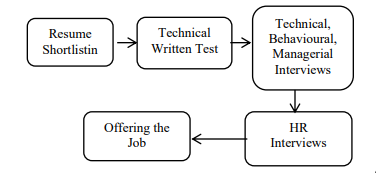
\includegraphics[width = 10 cm]{1.png}
\caption{Basic Job Hiring Process.}
\end{center}
\end{figure}

\section{Resume Screening consists of 4 basic steps:}
\begin{itemize}
    \item {Selecting the resumes with the required credentials, i.e., 
only the resumes matching the required job description,
will be considered.}
    \item {Select the resumes with the desired skills, i.e., only the 
candidates who mentioned the skills that match the job 
role will be considered.}
    \item {Selecting the resumes customized for the job, i.e., 
considering the resumes that accurately match the job 
role.}
    \item {Checking the applicant's information, i.e., scanning all 
the candidate's information and considering which 
matches the job profile properly.}
\end{itemize}

\begin{figure}[h]
\begin{center}
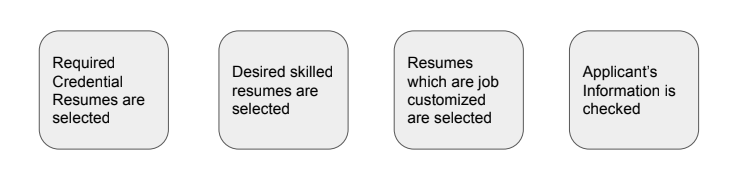
\includegraphics[width = 12 cm]{2.png}
\caption{ Steps involved in Resume Screening}
\end{center}
\end{figure}

Some of the most common difficulties encountered 
during the resume screening process
\begin{itemize}
    \item {Time Consuming-When there are a lot of resumes, it 
becomes more difficult.}
    \item{Hiring Quality-When there is a bulk of resumes, the
hiring quality suffers.}
    \item{Hiring Biases-Recruiters may be biased in favor of 
certain prospects.
}
    \item{Recruiter Experience-If, the recruiter, is unfamiliar 
with all of the job-related abilities, the screening 
procedure may be inefficient.}
    \item{Recruiters Search-If, a suitable applicant is located, 
recruiters may halt the search and skip the rest of the 
stack.
}
    \item{Unnecessary recruiter allocation-Separate recruiters 
should be assigned to the resume screening process, 
wasting time and resources.}
\end{itemize}


\section{Problem Statement}
\subsubsection{Volume of resume:}
The number of resumes received by a company is one of the biggest challenges. On average, there are about 250 resumes received for an open position, and 88\% of them tend to be unqualified. It means the recruiter has to spend enough time to cut the clutter, and finalise the 12\% of candidates. This amounts to close to 23 hours on average. The usual solution to this problem is the Applicant Tracking System (ATS), a must-have software for screening resumes in a company.

\subsubsection{Hiring Criteria:}
Sometimes, companies can set criteria for their hires or a framework to get their hiring process done. Even in the initial part when screening of resumes is taking place, it can prevent good candidates from getting filtered out. It should make companies vigilant about the resume screening process. Also, there is a need for revisiting the screening process consistently to ensure that the worthy candidates get the opportunities to enter the next round.



\chapter{SYSTEM ANALYSIS} %use UPPER CASE letters
\section{Existing Systems}
There are several existing systems and methodologies of resume screening techniques that are widely used . Here are some notable techniques:

\subsection{ Manual Screening}Screening of resumes is done by some of the company's employees who are going to recruit, i.e., every resume is checked individually, and if the resume is fit for the required job description, then the resume will be selected. It might be done based on the capabilities they seek, the
candidates' work experience, or other factors that are relevant
to the job profile.

\subsection {Resume Evaluation System based on AI}A Resume Screening Software is created using artificial intelligence, text mining, and processing algorithms. These algorithms filter and rank resumes based on specific keywords to identify which job applications recruiters should consider further.


\subsection{Resume Sorting using Artificial Intelligence} A Database is created to store job applicants' resumes. This system is trained using Artificial Intelligence to recognize the words separately from a resume. Some important keywords that fit the job description, like skills, education qualification, and so on, are given to the system separately through some other files. The system is trained to scan the resumes and search for the separately given keywords. 

\subsection{Resume Sorting using ML} The system
starts by cleansing all the unimportant information in the
resumes, such as numbers, special characters, single-letter
words, etc. They are then placed in one data set where the
data is split into tokens using NLTK tokenizes.

\subsection{Resume Screening using Machine Learning} The screening process should begin with removing garbage terms. The remaining words are then screened, and skill points are granted. And the skill points will be assigned in the appropriate order. Finally, a graph will be displayed due to the skill points, allowing eligible
candidates for the job role to be selected.

\subsection{Resume Screening Using Deep Learning}The data set primarily has 2 columns in this project. They are Category and Resume. The category represents the fields like Java, Database,
Blockchain, and so on. We must allocate the resume into one of the categories by utilizing it as input.

\subsection{Resume Screening Using Python}It was created using the Deep Learning method and learns from its prior data. Using the specified categories and resumes, the screening process has begun. Each resume is taken in and screened, then used to create output for that specific resume. 


\section{Literature Review}

\par In the paper[1], Manual screening, it abstracting the file only in PDF 
format,so here there is no other options to add up the different kind 
of file formats which is named like docx, zip so on. Manual resume screening refers to the process of reviewing and evaluating job applicants' 
resumes or CVs by human recruiters or hiring managers. It is a crucial step in the recruitment and selection process that helps identify qualified candidates for a particular job position.
During manual resume screening, recruiters typically follow a set of predefined criteria or job requirements to assess each applicant's qualifications, skills, and experience. The process involves analyzing the content of the resume to determine whether the candidate possesses the necessary qualifications and potential to succeed in the role.
Here are some key steps involved in manual resume screening:
\newline
Resume Collection: Resumes are collected through various channels such as job boards, company websites, career fairs, or employee referrals.
\newline
Initial Review: Recruiters go through the received resumes and conduct an initial scan to eliminate any clearly unqualified applicants. This scan is usually based on basic criteria like education level, relevant work experience, and key skills mentioned in the job description.
\newline
Skill Assessment: Recruiters then evaluate the candidate's skills and qualifications relevant to the job requirements. They look for specific keywords or phrases related to the required technical or soft skills to assess the candidate's suitability for the role.
\newline
Work Experience Evaluation: Recruiters carefully examine the candidate's work experience section to evaluate the relevance and depth of their previous roles. They assess the duration, job titles, responsibilities, and accomplishments to determine if the candidate's experience aligns with the job requirements.
\newline
Education and Certifications: The educational background and any relevant certifications mentioned in the resume are reviewed to ensure they meet the minimum requirements specified for the position.
\newline
Additional Qualifications: Recruiters assess any additional qualifications, such as language proficiency, leadership experience, or industry-specific certifications, that may be required for the role.
\newline
Formatting and Presentation: The resume's overall formatting, organization, and readability are considered to gauge the candidate's attention to detail and communication skills. A well-structured and error-free resume often receives more favorable consideration.
\newline
Applicant Ranking: Based on the evaluation, recruiters rank or score the resumes to prioritize the most promising candidates. This ranking helps determine which candidates will proceed to the next stage of the hiring process, such as interviews or assessments.
\newline
It's important to note that manual resume screening can be time-consuming, especially when dealing with a large number of applications. To streamline the process, some organizations may use applicant tracking systems (ATS) or resume screening software to automate the initial screening and filter out resumes that don't meet certain criteria before manual review.
\newline
Manual resume screening plays a crucial role in identifying potential candidates for further evaluation, ensuring that only the most qualified individuals proceed in the hiring process.
The problem for the paper is that it is time consuming error ineffcient and having alot of pressure. The solution which is give into the paper is resume is checked by a hiring team which is only focusing for the resume checking by individually. The drawback for the paper is that due to many resumes and little time availability for procesing it is very diffliculty and many resumes can be rejected without given an proper attention to the profile.
\bigskip
\par In the paper[2], manual screening with the help of web application is an another type of screening process that is used to be assigned earlier. Manual screening of resumes with the help of the web involves using online platforms and resources to review and evaluate job applicants' resumes or CVs. Here's a brief overview of the process:
\newline
Resume Submission: Candidates submit their resumes or CVs through online platforms like job boards, company websites, or recruitment portals.
\newline
Resume Parsing: The submitted resumes are often processed through resume parsing software, which extracts relevant information and structures it into a standardized format. This helps to categorize and organize the resumes for easier review.
\newline
Online Search: Recruiters may conduct online searches to gather additional information about the candidates. They might search for the candidate's name, review their social media profiles (e.g., LinkedIn), or explore professional networking sites to gain insights into their professional background and online presence.
\newline
Applicant Tracking Systems (ATS): Many organizations utilize ATS software to manage the hiring process. Recruiters may use the ATS to filter resumes based on predefined criteria such as keywords, qualifications, or location. The system can narrow down the pool of applicants, making it more manageable for manual screening.
\newline
Review and Evaluation: Recruiters review the resumes manually, considering various aspects such as education, work experience, skills, achievements, and qualifications. They assess whether the candidate's background aligns with the job requirements and evaluate the overall quality and presentation of the resume.
\newline
Online Reference Checks: Recruiters may conduct online reference checks by reaching out to the provided references through email or professional networking platforms. They might inquire about the candidate's performance, skills, and work ethic to gather additional insights.
\newline
Communication: If recruiters find potential matches during the manual screening, they may reach out to the candidates via email or through the contact information provided in their resumes. This communication may involve requesting additional information, scheduling interviews, or inviting candidates for further assessments.
\newline
Shortlisting and Ranking: Recruiters rank or shortlist the candidates based on their evaluation. This ranking helps determine which candidates will proceed to the next stages of the hiring process, such as interviews or assessments.
\newline
By leveraging the web, recruiters can access a larger pool of candidates and gather more information to aid in the screening process. However, it's essential to handle the information obtained from online sources ethically and with respect for privacy regulations.
\newline
It's worth noting that while the web can assist in streamlining certain aspects of resume screening, the final evaluation and decision-making process usually relies on the judgment and expertise of human recruiters or hiring managers.
\newline
The problem which is observed in the paper is that it is time consuming, inefficient, error and having alot of pressure.
The resume is checked with the help of the web application.
The major drawback is that can be miss out some datas and can create a bug due to heavy traffic because it is overflowing over the internet.
\bigskip
\par In the paper[3] screening with automatic scoring is fully in the basic of calculating the score which the candidate has occured.
Resume screening with automatic scoring involves using software or algorithms to assess and score resumes based on predefined criteria. Here's a brief explanation of the process:
\newline
Resume Collection: Resumes are collected through various channels, such as online job portals, company websites, or recruitment platforms.
\newline
Resume Parsing: The collected resumes are processed using resume parsing software, which extracts relevant information and structures it into a standardized format. This helps in organizing the data for automated analysis.
\newline
Predefined Criteria: The hiring organization establishes predefined criteria or job requirements that the resumes will be evaluated against. These criteria may include qualifications, skills, experience, education, certifications, and other relevant factors.
\newline
Automated Analysis: The resume screening software or algorithm analyzes the resumes based on the predefined criteria. It scans the resume content, including the text and keywords, to identify matches or discrepancies with the job requirements.
\newline
Scoring System: The software assigns scores or rankings to the resumes based on the degree of alignment between the resume and the predefined criteria. Each criterion may have a different weight or importance, and the algorithm calculates an overall score based on these factors.
\newline
Elimination or Shortlisting: Resumes that do not meet the minimum scoring threshold or fail to fulfill essential criteria may be eliminated at this stage. On the other hand, resumes that receive high scores and meet the desired criteria may be shortlisted for further evaluation.
\newline
Human Review: After the automated scoring, the shortlisted resumes are usually reviewed manually by recruiters or hiring managers. They consider the automated scores as a reference but also take into account other subjective factors that may not be captured by the software, such as the quality of writing, unique accomplishments, or relevant contextual information.
\newline
Final Selection: The resumes that pass the automated scoring and subsequent manual review are considered for further stages of the hiring process, such as interviews, assessments, or background checks.
\newline
Automated scoring in resume screening aims to streamline the initial screening process by efficiently handling large volumes of resumes. It helps recruiters and hiring teams save time and focus on the most promising candidates. However, it's important to note that automated scoring is not a foolproof method and should be used as a tool to assist human decision-making rather than as a substitute for it.
\newline
The problem is that it is time consuming,formation of errors, inefficient, having a lot of pressure. The solution which is given for this paper is to analyzebased on education qualification. The drawback for this paper is that missing out skilled candidates.Those who are having skillful mind set for certain kind of specific tasks.
\bigskip
\par In the paper[4],Resume Screening with the help of cloud database 
here the paper is storing all kind of datas in to the cloud database.
Resume screening with the help of a cloud database involves utilizing cloud-based technologies and databases to store, access, and analyze resumes during the screening process. Here's a brief explanation of how it works:
\newline
Cloud Storage: Resumes are stored in a cloud-based database or storage system. This allows for easy and centralized access to resume data from anywhere with an internet connection. Resumes can be securely uploaded and stored in the cloud, eliminating the need for physical storage or local servers.
\newline
Resume Parsing and Data Extraction: When resumes are uploaded to the cloud database, resume parsing technology can be applied to extract relevant information from the resumes and structure it in a standardized format. This parsing process helps categorize and organize the resume data for efficient retrieval and analysis.
\newline
Data Indexing and Search: The cloud database indexes the parsed resume data, making it searchable. Recruiters or hiring managers can use search queries or filters to quickly retrieve resumes based on specific criteria such as skills, experience, education, or keywords related to the job requirements.
\newline
Automated Screening Algorithms: Resume screening algorithms can be implemented within the cloud database to automatically analyze and evaluate resumes based on predefined criteria. These algorithms can scan the parsed resume data and identify matches or discrepancies with the desired qualifications and skills. The screening algorithms may assign scores or rankings to the resumes based on the degree of alignment with the job requirements.
\newline
Collaboration and Accessibility: Cloud-based resume screening enables multiple recruiters or hiring team members to access and collaborate on the screening process simultaneously. They can review and provide feedback on resumes in real-time, share notes, and collaborate on shortlisting or ranking candidates. This improves efficiency and ensures a streamlined screening process.
\newline
Integration with Applicant Tracking Systems (ATS): The cloud database can be integrated with ATS software, allowing for seamless transfer of resume data between systems. This integration enables recruiters to manage the entire recruitment workflow, including resume screening, in a unified platform.
\newline
Data Security and Privacy: Cloud databases provide robust security measures to protect the sensitive resume data. Access controls, encryption, and regular backups are implemented to ensure data privacy and integrity. Compliance with relevant data protection regulations, such as GDPR, is essential to maintain confidentiality and protect candidate information.
\newline
By leveraging cloud databases, resume screening becomes more efficient, scalable, and collaborative. The centralized storage, parsing capabilities, search functionality, and automated screening algorithms enhance the speed and accuracy of the screening process. Recruiters can access and analyze resumes from anywhere, collaborate effectively, and make data-driven decisions for shortlisting candidates.
The problem which is given is same as mentioned in above all papers,The solution which is given for that is 
storing the datas on the cloud so that it can easily sort it out whenever the recruitment team needs. The drawback is that it can have a high formation of bugs,due to the use of internet usage.
\newline
\par In the paper[5]Resume screening based on experience, is fully based on the candidate experience certification process.
Resume screening based on experience involves evaluating and assessing job applicants' work history and relevant experience to determine their suitability for a particular role. Here's a brief explanation of how resume screening based on experience typically works:
\newline
Job Requirements: Recruiters establish the necessary qualifications and experience criteria for the position. This includes factors such as minimum years of experience, specific industry experience, job-specific skills, and relevant accomplishments.
\newline
Work History Evaluation: Recruiters carefully review the candidate's work history section in the resume to assess their past employment experiences. They analyze factors such as job titles, company names, job duration, and responsibilities to gain insights into the candidate's professional trajectory.
\newline
Relevance to the Role: Recruiters evaluate the relevance of the candidate's work experience to the requirements of the job. They assess whether the candidate has held positions that align with the job's responsibilities, industry, or desired skills. They also consider the depth and breadth of experience in the relevant field.
\newline
Chronological Order: Recruiters examine the chronological order of the candidate's work history. They look for any employment gaps or inconsistencies that may need clarification. They also assess the progressive nature of the candidate's career and the level of responsibility held in each role.
\newline
Accomplishments and Responsibilities: Recruiters focus on the candidate's accomplishments and responsibilities within their previous roles. They assess the candidate's impact, achievements, and contributions to projects, teams, or organizations. They look for specific examples that demonstrate relevant skills, such as leadership, problem-solving, or project management.
\newline
Quantifiable Results: Recruiters pay attention to any quantifiable results or metrics mentioned in the resume. These could include sales figures, revenue growth, cost savings, or other measurable outcomes that highlight the candidate's achievements and effectiveness in previous roles.
\newline
Career Progression: Recruiters assess the candidate's career progression and growth over time. They look for indications of increasing responsibility, promotions, or transitions to higher-level roles. A clear and upward trajectory can demonstrate the candidate's ability to take on challenges and grow professionally.
\newline
Industry Relevance: Recruiters consider the candidate's experience within the specific industry or related sectors. They evaluate whether the candidate has the necessary knowledge, familiarity with industry-specific processes, or understanding of relevant regulations.
\newline
Additional Factors: Recruiters also take into account other factors, such as the reputation of previous employers, the size of organizations the candidate has worked in, and any notable projects or clients they have been associated with.
\newline
Based on the evaluation of the candidate's experience, recruiters determine whether the candidate meets the required level of expertise and is likely to succeed in the role. Candidates with relevant, in-depth experience that closely matches the job requirements are typically given higher consideration during the resume screening process.
The problem is same as mentioned in all the above papers,The solution which is given to this paper is analyze based on eperiences of candidates,The major drwaback for this paper is that they will miss out the freshers and skilled peoples, who doesnt have any kind of experiences in any field.
\bigskip
\par In the paer[6],Resume screening based on AWS methodology,Here the Problem is having same as above mentioned all papers.
Resume screening using Amazon Web Services (AWS) involves leveraging AWS services and tools to enhance the resume screening process. Here's a brief explanation of how it can be implemented:
\newline
Data Storage and Management: AWS offers scalable and secure cloud storage solutions, such as Amazon S3 (Simple Storage Service) or Amazon RDS (Relational Database Service). Resumes can be stored in these services, ensuring easy accessibility, durability, and high availability.
\newline
Resume Parsing: AWS provides services like Amazon Textract or Amazon Comprehend, which can be used to extract structured data from resumes automatically. These services leverage machine learning algorithms to parse resumes and extract information such as candidate names, contact details, work experience, education, and skills. This parsing process saves time and eliminates manual data entry.
\newline
Resume Indexing and Search: AWS services like Amazon Elasticsearch or Amazon CloudSearch can be used to index the parsed resume data, making it searchable. Recruiters can query the indexed data using search queries or filters to find resumes based on specific criteria, such as skills, experience, or education.
\newline
Natural Language Processing (NLP): AWS offers NLP services like Amazon Comprehend or Amazon Lex, which can be used to analyze resume content. These services can extract key phrases, entities, or sentiments from resumes, helping recruiters gain deeper insights into the candidates' qualifications, accomplishments, and experience.
\newline
Automated Screening and Scoring: AWS allows the development and deployment of custom machine learning models using services like Amazon SageMaker. Recruiters can build models to automatically screen and score resumes based on predefined criteria. Machine learning algorithms can analyze the parsed resume data, compare it against job requirements, and assign scores or rankings to candidates based on their qualifications and relevance.
\newline
Cloud Computing Power: AWS provides scalable and powerful computing resources through services like Amazon EC2 (Elastic Compute Cloud) or AWS Lambda. These resources can be leveraged to process large volumes of resumes efficiently and perform resource-intensive tasks, such as running complex algorithms or conducting extensive data analysis.
\newline
Integration with Applicant Tracking Systems (ATS): AWS services can be integrated with existing ATS platforms, allowing seamless data transfer between systems. This integration ensures a smooth flow of resume data, including parsed information, scoring results, and other relevant details, to streamline the overall recruitment workflow.
\newline
Data Security and Compliance: AWS provides robust security features and compliance certifications, ensuring the protection and privacy of candidate data. Encryption, access controls, and data backup mechanisms help maintain data security and meet regulatory requirements.
\newline
By utilizing AWS services, resume screening processes can be enhanced with automation, scalability, and advanced analysis capabilities. This can result in improved efficiency, accurate candidate assessment, and a more streamlined recruitment process.
The solution which is given to the paper is that utilizing AWS method The drawback is that it only focusing the AWS data.


%\begin{table*}[h]
 % \caption{LITERATURE SURVEY}
 %   \centering
%    \begin{tabular}{|p{3cm}|p{3cm}|p{3cm}|p{3cm}|}
 %   \hline
 %       \textbf{PAPER NAME} & \textbf{PROBLEMS} & \textbf{SOLUTION} & \textbf{DRAWBACK}  \\
 %       \hline
  %       Image denoising via sparse and redundant representations over learned dictionaries. IEEETransactions on Image Processing & To de-noising the input image and obtain clear image as output
%& Basedon sparse and redundant representations over trained dictionaries, Using the K-SVD algorithm. 
%& For the higher noise power experiments, this approach deteriorates faster and achieves weaker results
 \\
%         \hline
 %       Deep joint demosaicking and denoising. ACM Transactions on Graphics, 35(6), 2016
 %& To demosaicking and denoising the input image.
% & Introduce a new data-driven approach and train a deep neural network on a large corpus of images insteadof using hand-tuned filters.& The data produced are corrupted and produce inaccurate output.. \\
 %        \hline
  %      Adaptive multicolumn deep neural networks with application to robust image denoising. In NIPS, 2013
 %& To improve image quality and reomve the noises from images
 %& Stacked sparse denoising auto-encoders (SSDAs) are used to enhance the image and denoising purpose
% & Doesn’t works on color images it shows better results in black and white images
\\
 %        \hline
  %       RENOIR – A dataset for real low light image noise reduction. arXiv:1409.8230, 2014. 2-J. Anaya and A. Barbu.
%& image denoising procedure takes a noisy image as input and outputs an image where the noise has been reduced
% &A well algorithm named RENOIR is used to rectify this problem
% & Complicated algorithm used .Low efficiency\\

 %        \hline
  %      Trainable nonlinear reaction diffusion:. IEEE Transactions on Pattern Analysis and Machine
%Intelligence, 39(6), 2017
 %& To restore image from noisy and blurred ones.
% & Proposed a flexible learning framework based on learning optimal nonlinearreaction diffusion models. It's is know as TNRD approach 
% & This approach is not suitable for evry datasets .\\
 % \hline
 %   \end{tabular}
  %  \label{tab:my_label}
%\end{table*}

%\begin{table*}[h]
  
  %  \centering
 %   \begin{tabular}{|p{3cm}|p{3cm}|p{3cm}|p{3cm}|}
   % \hline
    %    \textbf{PAPER NAME} & \textbf{PROBLEMS} & \textbf{SOLUTION} & \textbf{DRAWBACK}  \\
    %    \hline
     %Image denoising by sparse 3-D transform-domain collaborative filtering. IEEE Transactions on Image Processing, 16(8), 2007.
 %& To denoise the input image
%& By grouping 2D image into 3D array and collaborative filtering of these 3D groups. And using image de-noising algorithm
%&Color image de-noising is non-trivial because it  do not apply the grayscale BM3D independently.The grouping is done only once.
 \\
 % \hline
 %Fast efficient algorithm for enhancement of low lighting video. In IEEE International Conference on Multimediaand Expo 2017 & Enhancement of low light lighting video
%& The algorithm works by first inverting an input low-lighting video and then applying an optimized image de-haze algorithm on the inverted video. 
 %& The SNR ratio is not timal and the time taken to process is very big.


 %\\
 %\hline
 %Image denoising: Can plain neural networks compete with BM3D.H. C. Burger, C. J. Schuler, and S. Harmeling
 %& The noises present in images are reduced and better low light images.
%& BM3D is a  algorithm could we also  learn an image denoising procedure purely from training examples consisting of pairs of noisy and noise free patches
%& MLP is tailored to a single level of noise and does not generalize well to other noise levels compared to other denoising methods


 %\\
 %\hline
  %Photographic image synthesis withcascaded refinement networks. In ICCV, 2017.-Q. Chen and V. Koltun.
 %& To improve image quality and reomve the noises from images
 %& Approach produces an image with photographic appearance that conforms to the input layout
%& This system some time illustrates less efficient output and the SNR ratio is some time high


 \\
% \hline
 % Fast image processing with
%fully-convolutional networks. In ICCV, 2017.
 %& To increase the quality and eliminate the effect of atmospheric shattering.
%& Approximate the operators using convolutional network.
% & its approximationaccuracy is low and limited support for recovering the lost high-frequency content during upsampling.


 \\
 %       \hline
  %  \end{tabular}
   % \label{tab:my_label}
%\end{table*}


\section{Proposed System}
Resume Screening is the primary step in the hiring process. It evaluates the candidates' resumes and determines whether they are qualified for a role based on their education, skill sets, technical stuff, experience, and other information captured in their resume. To make it simple, it's a form of pattern that matches the job requirement and the candidate's qualifications based on their resume. It is a crucial step in the process of hiring. It is the step in which a decision is made to move the candidate to the next level or not. There are multiple processes to perform resume screening. Among all the processes, traditional resume or manual screening is the largest followed, even today. But usually, companies receive thousands of resumes for job applications, which consumes a lot of time and effort. In addition to this, many errors may arise due to human involvement. Multiple ways were introduced to cover all these cons to performing this resume screening process. Various technologies, including Artificial Intelligence and Machine Learning, were involved in searching for solutions.
\newline
\par Resume screening software (also known as candidate screening software) helps recruitment and talent acquisition departments increase efficiency. It does that by organizing all the resumes received for each role so that the team is able to prioritize the candidates they want to invite to the interview process. Typically, a resume screening tool will determine the best applicants for a role based on keyword search results or answers to specific questions.

\chapter{SYSTEM DESCRIPTION AND OPERATION}  %use UPPER CASE letters



\section{System Architecture}

The first process of our project is to develop webpage for our resume screening with the help of HTML,the front end are created and formatted the design how it should appear in the processs, the main ultimate task  of this project is to upload the pdf file format of the resume which is to be screened.and the uploaded pdf format file is extarcted and will clean up the text formats from the  uploaded resume.after cleaning the pdf it will gone for the dictionary process to analyse the file, after going to that process the final step is to calculate the scores that is been calculated by the software and the uploaded pdf client will get the mail confirmation regarding the first process is completed and selected to the next process of interview scheduling.

\begin{figure}[h]
	\begin{center}
		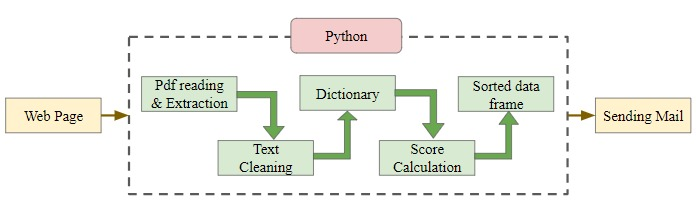
\includegraphics[width =15 cm]{arch.jpeg}
		\caption{System architecture}
		\label{ab}
	\end{center}
\end{figure}

\section{Phases of Resume Screening}
\subsection{Module 1}
\begin{figure}[h]
	\begin{center}
		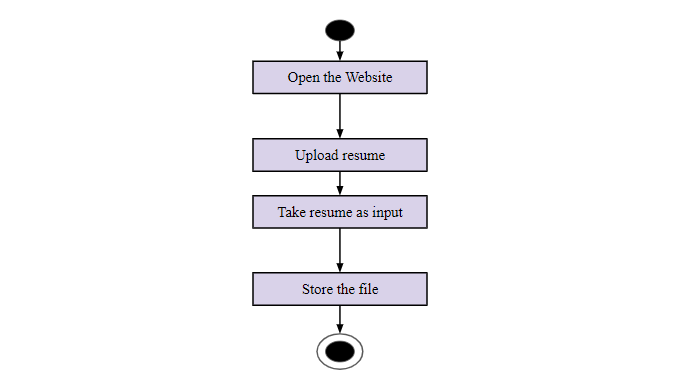
\includegraphics[width = 13 cm]{m1.png}
		\caption{Architecture of Module 1}
		\label{ab}
	\end{center}
\end{figure}


The candidates can only upload the resume which 
is in the format of PDF, into the website which we created with the help of the html. 
In to that created website the candidate need to upload the resume. Now the uploaded resume is taken as input process and it will performs it's further steps in next module.

\bigskip


\subsection{Module 2}

\begin{figure}[h]
	\begin{center}
		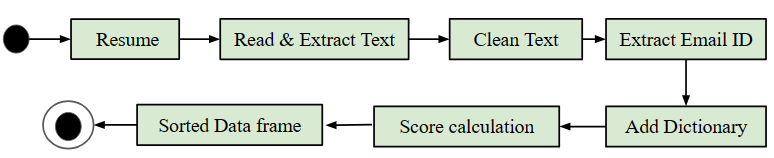
\includegraphics[width = 13 cm]{m2.png}
		\caption{Architecture of Module 2}
		\label{ab}
	\end{center}
\end{figure}


\bigskip
Now the uploaded resume is taken as input that as mentioned earlier in the module 1, and the next phase of the project is to take the resume that has been uploaded and it reads and extract the text from the uploaded resume. Here they only take the pdf files. After extraction of the text, the resume is cleaned, which means clearing all kind of unnecessary texts such as commas, bracket and all sorts of special symbols. As the special symbols are removed we add @ symbol for extracting the E-mail id from resume. 
\newline Then a dictionary is added where there would be keywords. The key terms included in each area of this dictionary were obtained through a research of the most common key terms included in industrial and system engineering job postings. This dictionary can be customized to add/remove key terms according to hiring managers criteria.
\newline
So when the extracted text words matches the words of keyword then the scores are appended. With the scores a calculated a sorted data frame would be created. With the help of sorted data frame a pie chart would be created. 

\subsection{Module 3}
\begin{figure}[h]
	\begin{center}
		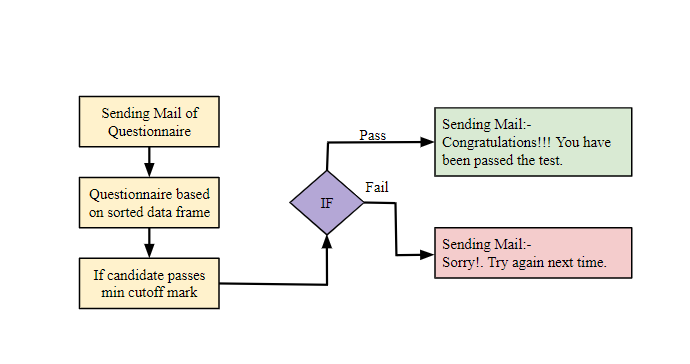
\includegraphics[width = 13 cm]{m3.png}
		\caption{Architecture of Module 3}
		\label{ab}
	\end{center}
\end{figure}

\bigskip
The sorted data frame that has been already calculated in module 2 would be taken out to check the condition that the company required. The condition would be like: "if a candidates resume has a pass score in a particular slice of the pie chart then an automated mail would be send to the candidates". The pass score in particular slice is arranged by the company.

\bigskip\bigskip
\bigskip\bigskip
\bigskip\bigskip
\bigskip

%\bigskip\bigskip\bigskip

%\section{OVERALL ALGORITHM}
%\begin{enumerate}
%\item
%\item
%\item
%\item Output Generation: The final enhanced image is generated as the output of the dark image enhancement process. This image exhibits improved visibility, enhanced details, and better overall quality compared to the original dark image.
    
%\end{enumerate}
\bigskip
%\section{USER INTERFACE}  %use UPPER CASE letters
%UI stands for User Interface. It refers to the visual elements, controls, and interactions that allow users to interact with and control a software application, website, or system. UI encompasses the design of graphical user interfaces (GUIs), web interfaces, mobile app interfaces, and other forms of digital interfaces.

%\begin{figure}[h]
%	\begin{center}
%		\includegraphics[width =12 cm]{UI.jpeg}
%		\caption{User Interface}
%		\label{ab}
%	\end{center}
%\end{figure}
%\bigskip
%\bigskip
%\bigskip
%\bigskip\bigskip
%\bigskip


\chapter{SYSTEM SPECIFICATION}

%\section{HARDWARE REQUIREMENTS}
%\begin{enumerate}
%\item  Processor: A powerful processor is essential for handling the computational demands of image enhancement algorithms. A multi-core processor with a high clock speed will help improve the performance and speed of the image enhancement operations. Here we used  intel i5 gen 11 for the implementation.

%\item Memory (RAM): Sufficient memory is required to load and process images efficiently. The amount of RAM you need depends on the size and complexity of the images you plan to process. For image enhancement tasks, it is recommended to have a minimum of 8 GB of RAM, but higher amounts, such as 16 GB or more, will be beneficial for processing larger images or handling multiple requests concurrently. our system contains 8GB RAM.

%\item Storage: Adequate storage space is necessary to store the images and any associated data or databases. The amount of storage you need will depend on the anticipated number and size of the images you expect to handle. Additionally, if you plan to store user-uploaded images or processed images, you will need enough storage capacity to accommodate them.Our system has 1TB HDD and 256 SSD.

%\item Graphics Processing Unit (GPU): While not mandatory, a dedicated GPU can significantly accelerate image processing tasks, especially for computationally intensive enhancement algorithms. GPUs with CUDA support can be leveraged to accelerate deep learning-based image enhancement models or other GPU-accelerated algorithms. However, if your webpage primarily uses lightweight enhancement techniques, a dedicated GPU may not be necessary. Our system contains dedicated NVIDIA GEOFORCEX.

%\item Monitor/Display: Although not directly related to hardware requirements, having a high-resolution monitor or display is helpful for previewing and evaluating the enhanced images during development and testing.
%\end{enumerate}

\section{Software Requirements}

For the implementation of our project we choose visual studio code as our IDE. Visual Studio Code, also commonly referred to as VS Code, is a source-code editor made by Microsoft with the Electron Framework, for Windows, Linux and macOS. Features include support for debugging, syntax highlighting, intelligent code completion, snippets, code refactoring, and embedded Git. Users can change the theme, keyboard shortcuts, preferences, and install extensions that add functionality.

\subsection{Why visual studio code}


Visual Studio Code (VS Code) is a lightweight, free source code editor developed by Microsoft. It has gained immense popularity among developers due to its extensive features, flexibility, and wide range of extensions. Here's an overview of Visual Studio Code:
\begin{enumerate}
\item Cross-platform and Lightweight: VS Code is available for Windows, macOS, and Linux, ensuring compatibility across different operating systems. It is designed to be lightweight, providing fast performance while consuming minimal system resources.

\item Intuitive User Interface: VS Code has a clean and intuitive user interface that maximizes the coding space. It offers a customizable layout, allowing users to adjust the view and position of panels, sidebars, and editors according to their preferences. The user interface is designed to enhance productivity and provide a distraction-free coding environment.

\item Extensive Language Support: VS Code provides support for a wide range of programming languages out of the box, including popular ones like JavaScript, Python, Java, C++, and many more. It offers syntax highlighting, code snippets, and intelligent code completion, making it easier to write code and catch errors quickly.

\item Integrated Terminal: VS Code includes an integrated terminal that allows developers to run commands, execute scripts, and interact with the command-line interface without leaving the editor. The terminal can be customized and supports multiple instances, making it convenient to work with different environments or tools.

\item Git Integration: VS Code has excellent Git integration, enabling developers to perform version control tasks within the editor. It provides features like Git staging, commit history, branch management, and conflict resolution. Users can visually track changes, compare file revisions, and collaborate with teammates using version control.

\item Powerful Editing Features: VS Code offers a rich set of editing features to enhance productivity. These include intelligent code completion, code refactoring, formatting, find and replace, multiple cursors, code folding, and more. It supports customizable keyboard shortcuts, allowing users to optimize their workflow and increase efficiency.

\item Integrated Debugging: VS Code provides integrated debugging capabilities for various programming languages. It allows developers to set breakpoints, step through code, inspect variables, and view call stacks, providing an efficient debugging experience. Debugging configurations can be customized to match specific project requirements.

\item Extensibility with Extensions: VS Code has a vibrant ecosystem of extensions contributed by the community. These extensions enhance the editor's functionality by adding support for additional languages, frameworks, and tools. They provide features like linters, code formatters, language servers, live server preview, and integrations with cloud platforms and build systems.

\item Integrated Package Manager: VS Code includes a built-in package manager called the Extension Marketplace. It allows users to discover, install, and manage extensions directly from within the editor. The marketplace offers a wide range of extensions to customize and extend the functionality of VS Code.

\item  Live Collaboration: VS Code supports live collaboration through extensions like Live Share. It enables developers to collaborate in real-time, share their coding sessions, and work together on the same codebase, irrespective of their physical location. This feature facilitates pair programming, code reviews, and remote collaboration.
  
\end{enumerate}
Visual Studio Code provides a powerful, user-friendly, and customizable environment for developers. Its extensive feature set, flexibility, and strong community support make it a popular choice for a wide range of programming tasks, from small scripts to large-scale projects.

\chapter{SOFTWARE DESCRIPTION}
\section{Languages Used }

\subsection{Python}
The code to implement this project is done with the language Python.
Python is a popular high-level programming language known for its simplicity, readability, and versatility. It was created by Guido van Rossum and first released in 1991. Python emphasizes code readability and allows programmers to express concepts in fewer lines of code compared to other programming languages. It has gained widespread adoption in various domains, including web development, data analysis, scientific computing, artificial intelligence, and automation.

Here are some key features and aspects of Python:
\begin{enumerate}
\item  Syntax and Readability: Python's syntax is designed to be intuitive and easy to read. It uses indentation to define blocks of code, making it visually distinct. This feature encourages developers to write clean and readable code.

\item  Interpreted Language: Python is an interpreted language, which means it does not require a compilation step before execution. The interpreter reads and executes the code line by line, allowing for rapid development and testing.

\item  Multi-paradigm: Python supports multiple programming paradigms, including procedural, object-oriented, and functional programming. This flexibility allows developers to choose the best approach for their project.

\item  Large Standard Library: Python comes with a vast standard library that provides numerous modules and packages for common tasks such as file I/O, networking, database access, and more. The standard library reduces the need for external dependencies and makes it easier to get started with various programming tasks.

\item  Third-Party Libraries: Python has a rich ecosystem of third-party libraries and frameworks that extend its capabilities. These libraries cover a wide range of domains, including web development (e.g., Django, Flask), data analysis (e.g., NumPy, pandas), scientific computing (e.g., SciPy), machine learning (e.g., TensorFlow, PyTorch), and more. This extensive collection of libraries makes Python suitable for various applications.

\item  Platform Independence: Python is a cross-platform language, meaning it can run on different operating systems such as Windows, macOS, and various Linux distributions. This portability makes it easier to develop and deploy applications across different environments.

\item  Integration and Extensibility: Python can easily integrate with other languages like C, C++, and Java, allowing developers to leverage existing code and libraries. It offers interfaces and tools for extending Python with native code for performance-critical tasks.

\item Community and Support: Python has a large and active community of developers who contribute to its growth and provide support through online forums, documentation, and open-source projects. This vibrant community ensures that Python remains up to date and well-supported.
\end{enumerate}

Python's versatility and ease of use have made it a popular choice for beginners learning to program, as well as for experienced developers working on complex projects. Its simplicity and expressiveness make it an excellent language for rapid prototyping, scripting, and building scalable applications.

\subsubsection{Python Flask-Framework}
Flask is a lightweight web framework for Python that allows you to build web applications quickly and with minimal boilerplate code. It was developed by Armin Ronacher and released in 2010. Flask is known for its simplicity, flexibility, and ease of use, making it a popular choice for web development.

Here are some key features and aspects of Flask:
\begin{enumerate}
  
\item  Microframework: Flask is considered a microframework because it focuses on simplicity and minimalism. It provides the core functionality needed for web development, such as routing, request handling, and template rendering, without imposing strict architectural patterns or adding unnecessary layers of abstraction. This lightweight approach gives developers more freedom to structure their applications according to their preferences.

\item  Routing and View Functions: Flask uses a decorator-based syntax to define routes and associate them with view functions. A route is a URL pattern that maps to a specific function. When a user accesses a particular URL, Flask invokes the associated view function to generate the response. This routing mechanism allows you to define different routes for various parts of your application and handle different HTTP methods (GET, POST, etc.) on those routes.

\item Template Engine: Flask includes a template engine called Jinja2, which enables you to generate HTML dynamically. Jinja2 allows you to separate the presentation logic from the application's business logic by defining templates with placeholders (variables) and control structures (loops, conditionals). You can pass data from your views to templates to render dynamic content.

\item  HTTP Request and Response Handling: Flask provides an easy-to-use API for handling HTTP requests and generating responses. You can access request data, such as form input, query parameters, and headers, using Flask's request object. Likewise, you can generate responses with different content types (HTML, JSON, etc.) using Flask's response object or by returning values directly from view functions.

\item  Extensions and Modularity: Flask follows a "micro but expandable" philosophy. While it provides a minimal core, you can extend its functionality using various Flask extensions. These extensions add extra features like database integration, authentication, form validation, and more. Flask extensions are developed by the community and can be easily integrated into your Flask applications.

\item  Development Server and Debugging: Flask includes a built-in development server that simplifies the testing and debugging process. It automatically reloads the server when you modify your code, allowing you to see the changes immediately. Additionally, Flask provides a robust error handling mechanism that displays detailed error messages and a debugger to help identify and fix issues during development.

\item Integration with Other Technologies: Flask seamlessly integrates with other Python libraries and tools, making it a versatile choice for web development. You can easily use Flask with popular database systems like SQLite, MySQL, or PostgreSQL, and integrate it with ORMs (Object-Relational Mappers) such as SQLAlchemy. Flask can also work well with front-end frameworks like React, Angular, or Vue.js to build single-page applications (SPAs).
  
\end{enumerate}
Flask's simplicity and flexibility make it a great option for small to medium-sized web applications, RESTful APIs, prototypes, and personal projects. It provides a solid foundation for web development in Python and allows developers to focus on their application's specific requirements without unnecessary complexity.

%\subsubsection{Why python?}
%Python is a popular programming language that offers several advantages for %implementing MirNet image enhancement techniques. Here are some reasons why %Python is commonly used in this context:
%\begin{enumerate}
 
%  \item Rich Ecosystem of Libraries: Python has a vast ecosystem of libraries and frameworks that provide extensive support for image processing, deep learning, and computer vision tasks. Libraries such as TensorFlow, PyTorch, and Keras offer powerful tools and APIs for building and training deep learning models like MirNet. These libraries provide pre-built functions, optimization algorithms, and utilities that simplify the implementation of complex image enhancement techniques.

 % \item Ease of Use and Readability: Python is known for its simplicity and readability, which makes it easier for researchers and developers to understand and modify existing code or develop new algorithms. Its clean and concise syntax allows for efficient prototyping and experimentation, enabling quick iteration and refinement of image enhancement techniques.

 % \item Extensive Community Support: Python has a large and active community of developers and researchers working on various image processing and computer vision projects. This vibrant community provides support through forums, online resources, and open-source contributions. The availability of resources, tutorials, and code examples makes it easier to learn and apply advanced techniques like MirNet for image enhancement.

  %\item Integration with Other Technologies: Python is well-suited for integrating with other technologies and frameworks commonly used in image enhancement workflows. It seamlessly integrates with popular software libraries like OpenCV, which provides a wide range of image processing and computer vision functions. Python also facilitates interoperability with data processing tools, visualization libraries, and web frameworks, enabling end-to-end image enhancement pipelines.

 % \item Prototyping and Experimentation: Python's interactive and dynamic nature allows for rapid prototyping and experimentation. With Python, it is relatively straightforward to load, preprocess, and visualize images, facilitating the exploration and analysis of image enhancement techniques. This flexibility and interactivity make Python an ideal choice for researchers and developers who need to iterate quickly and evaluate the effectiveness of different approaches.

 % \item Platform Compatibility: Python is a cross-platform language, meaning that code developed on one operating system can be easily executed on different platforms with minimal modifications. This flexibility is beneficial when deploying MirNet-based image enhancement techniques on various devices or systems, including desktops, servers, or embedded devices.
 
%\end{enumerate}
%\bigskip
%Overall, Python's rich ecosystem, ease of use, extensive community support, integration capabilities, prototyping advantages, and cross-platform compatibility make it a popular choice for implementing MirNet image enhancement techniques. It empowers researchers and developers to effectively leverage deep learning and image processing libraries, enabling the development of advanced and efficient algorithms for enhancing dark images.

\subsection{HTML}
HTML (Hypertext Markup Language) is the standard markup language used for creating the structure and content of web pages. It defines the elements and tags that structure the information displayed in a browser. Basic scripting language used by web browsers to render pages on the world wide web. HyperText allows a user to click a link and be redirected to a new page referenced by that link.

There is a range of HTML tags, they help you to design your web page. There are four required tags in HTML. These are html, title, head and body. The table below shows you the opening and closing tag, a description and an example.

There are three categories of HTML: transitional, strict, and frameset. Transitional is the most common type of HTML while the strict type of HTML is meant to return rules to HTML and make it more reliable. Frameset allows Web developers to create a mosaic of HTML documents and a menu system. It's the way web pages and email templates are coded so that text is formatted and images are added. Plain Text is regular text, with no formatting options such as bold, italics, underlines, or special layout options. HTML works alongside CSS and JavaScript to build interactive and visually appealing websites. Here's an overview of HTML:

\begin{enumerate}
\item  Document Structure: HTML documents are structured using a hierarchical format called the Document Object Model (DOM). The DOM represents elements as nodes in a tree-like structure. An HTML document starts with the <html> tag and contains a head section (<head>) for metadata and a body section (<body>) for the visible content of the page.

\item Elements and Tags: HTML elements are the building blocks of a web page. They are defined using tags, enclosed in angle brackets (<>). Tags are composed of an opening tag (<tag>) and a closing tag (</tag>), where the content resides. Some elements, known as empty elements, do not require a closing tag and are self-closing (<tag />). Examples of common HTML elements include headings (<h1>, <h2>, etc.), paragraphs (<p>), links (<a>), images (<img>), lists (<ul>, <ol>, <li>), and more.

\item Attributes: HTML elements can have attributes, which provide additional information about an element. Attributes are specified within the opening tag and consist of a name and a value (name="value"). Attributes define properties like the source of an image, the target of a link, the size of an input field, and more. Examples of attributes include src, href, class, id, alt, style, and data-* attributes.

\item Semantic Elements: HTML5 introduced a set of semantic elements that convey the meaning and structure of the content more accurately. These elements include <header>, <nav>, <section>, <article>, <aside>, <footer>, and more. Semantic elements provide better accessibility, improve search engine optimization (SEO), and help developers structure web pages in a more meaningful way.

\item Hyperlinks: HTML allows the creation of hyperlinks using the <a> (anchor) element. The href attribute specifies the URL to which the link points. Hyperlinks can be used to navigate within the same page, link to other pages, or link to external resources like images, documents, or videos. Additionally, HTML provides the ability to open links in a new window or tab using the target attribute.

\item Lists: HTML supports ordered (<ol>) and unordered (<ul>) lists. List items are defined using the <li> element, which is placed inside either an <ol> or <ul> element. Ordered lists display items with a numbering sequence, while unordered lists display items with bullet points. Nested lists can also be created by placing lists within lists.

\item Forms: HTML provides form elements (<form>, <input>, <textarea>, etc.) for capturing user input. Forms allow users to submit data to a server for processing. Various input types (text, email, password, checkbox, radio, etc.) and attributes (required, placeholder, disabled, etc.) can be used to define the behavior and appearance of form elements.

\item Multimedia: HTML supports the inclusion of multimedia content on web pages. The <img> element is used to display images, while the <audio> and <video> elements are used to embed audio and video files, respectively. These elements support different attributes for controlling playback, size, and alternative content.

\item Tables: HTML tables (<table>, <tr>, <td>) are used to organize data into rows and columns. Tables can be styled using CSS to enhance their appearance and improve readability. Additionally, HTML provides elements like <th> for table headers and attributes like colspan and rowspan for merging cells.
\end{enumerate}
HTML is continually evolving, with new versions introducing additional features and elements. It provides the foundation for web development, allowing developers to structure and present content in a standardized manner across different browsers and devices.

\subsection{CSS}
CSS (Cascading Style Sheets) is a fundamental technology used for styling and formatting web documents. It describes how HTML elements should be displayed on a web page, including their layout, colors, fonts, and other visual aspects. It allows one to adapt the presentation to different types of devices, such as large screens, small screens, or printers. CSS is independent of HTML and can be used with any XML-based markup language. 
CSS saves a lot of work. It can control the layout of multiple web pages all at once. External stylesheets are stored in CSS files.
CSS describes how elements should be rendered on screen, on paper, in speech, or on other media. 
CSS describes how elements should be rendered on screen, on paper, in speech, or on other media.
\newline
The name cascading comes from the specified priority scheme to determine which style rule applies if more than one rule matches a particular element. This cascading priority scheme is predictable. The CSS specifications are maintained by the World Wide Web Consortium.
There are 3 distinct methods for styling in CSS, Local style, Page-Level style, and External Styles. Each level of styling is given a different hierarchical priority (when to apply) and is used for different reasons. The 3 methods are further grouped into two categories. Namely Internal CSS and External CSS.
In CSS, a class is a group of elements that are the same or similar. You can have as many elements as you want in a class. And each element can be the member of multiple classes. Every class has CSS attributes (like color and font-size) that are specific to that class.
CSS works alongside HTML and JavaScript to create visually appealing and interactive web pages. Here's an overview of CSS:
\begin{enumerate}
  \item Separation of Style and Structure: CSS enables the separation of a web page's content (HTML structure) from its presentation (styling). This separation allows developers to define styles independently and apply them consistently across multiple web pages. It promotes clean code, easy maintenance, and the ability to update the visual appearance of a website without modifying the underlying HTML structure.

  \item Selectors and Declarations: CSS uses selectors to target specific HTML elements and apply styling rules. Selectors can be based on element types (e.g., h1, p), class names (e.g., .container, .highlighted), IDs (e.g., header, sidebar), and more. Once a selector is defined, you can specify one or more declarations, which consist of a property and a value. For example, you can set the color property to red, the font-size property to 16 pixels, or the background-image property to a specific image URL.

  \item Style Inheritance and Specificity: CSS employs a cascading nature, where styles can be inherited from parent elements and overridden by more specific rules. This cascading behavior allows for efficient and modular style definitions. However, when multiple conflicting styles are applied to the same element, CSS uses a specificity calculation to determine which style takes precedence.

  \item Layout and Positioning: CSS provides various layout and positioning options to control the arrangement of elements on a web page. These include properties like display (e.g., block, inline, flex), position (e.g., static, relative, absolute), float, margin, padding, and more. With these properties, you can create responsive designs, align elements, create columns, and control the flow of content.

  \item Responsive Design: CSS plays a crucial role in creating responsive web designs that adapt to different screen sizes and devices. Using CSS media queries, developers can define different styles based on the screen width, height, or other device-specific features. This allows the website layout and appearance to adjust dynamically, providing an optimal viewing experience on desktops, tablets, and mobile devices.

  \item Animations and Transitions: CSS provides support for animations and transitions, allowing developers to create engaging and interactive user experiences. With keyframes and animation properties, elements can move, change size, fade in/out, or perform other dynamic effects. Transitions enable smooth property changes over time, such as gradual color shifts or smooth transitions between layout states.

  \item Selectors and Pseudo-Classes: CSS offers a wide range of selectors to target specific elements or groups of elements. Additionally, pseudo-classes provide a way to target elements based on their state or position within the document. Examples of pseudo-classes include :hover, :active, :first-child, :nth-child(), and many more. These selectors and pseudo-classes enhance the control and interactivity of web pages.

  \item CSS Frameworks: To expedite web development and ensure consistent styling, developers often use CSS frameworks like Bootstrap, Foundation, or Bulma. These frameworks provide pre-designed CSS components, grids, and stylesheets that can be easily integrated into a project, simplifying the styling process and ensuring a cohesive visual design.
\end{enumerate}
\bigskip
CSS is continuously evolving, and new features and enhancements are regularly introduced to the language. With CSS, developers have powerful tools to control the presentation and styling of web pages.

\section{Installation}
\subsection{Install Visual Studio Code}
\begin{enumerate}
    \item Step 1: Visit the official website of the Visual Studio Code using any web browser like Google Chrome, Microsoft Edge, etc.
\item Step 2: Press the “Download for Windows” button on the website to start the download of the Visual Studio Code Application.
\item Step 3: When the download finishes, then the Visual Studio Code icon appears in the downloads folder.
\item Step 4: Click on the installer icon to start the installation process of the Visual Studio Code.
\item Step 5: After the Installer opens, it will ask you for accepting the terms and conditions of the Visual Studio Code. Click on I accept the agreement and then click the Next button.
\item Step 6: Choose the location data for running the Visual Studio Code. It will then ask you for browsing the location. Then click on Next button.
\item Step 7: Then it will ask for beginning the installing setup. Click on the Install button.
\item Step 8: After clicking on Install, it will take about 1 minute to install the Visual Studio Code on your device.
\item Step 9: After the Installation setup for Visual Studio Code is finished, it will show a window like this below. Tick the “Launch Visual Studio Code” checkbox and then click Next.
\item Step 10: After the previous step, the Visual Studio Code window opens successfully. Now you can create a new file in the Visual Studio Code window and choose a language of yours to begin your programming journey!
\end{enumerate}

\subsection{Install Python}
\begin{enumerate}
\item Install Python from python.org
\item You can typically use the Download Python button that appears first on the page to download the latest version
\item While installing python make sure that you install pip along with it
\end{enumerate}

\subsection{Verify the Python installation}
\begin{enumerate}
    \item To verify that you've installed Python successfully on your machine, run the following command
\item Open a command prompt and run the following command:
py -3 --version
\item If the installation was successful, the output window should show the version of Python that you installed.
\end{enumerate}

\subsection{Install Flask}
\begin{enumerate}
    \item Step 1: Install Virtual Environment
    \item Step 2: Create an Environment
    \item Step 3: Activate the Environment
    \item Step 4: Install Flask
    \item Step 5: Test the Development Environment
\end{enumerate}

\subsection{Code}
\begin{enumerate}
    \item Copy the code and download required libraries
pip3 install -r requirements.txt  
\item If pip doesn't work, then upgrade pip using following command:
py -m pip install --upgrade pip
\end{enumerate}

\subsection{Run the code}
\begin{enumerate}
    \item First activate the environment, to actiavte the environment:
C:\users\Documents\Source\resume-screener\<environment name>\Scripts\activate
\item After the environment is activated get the path back to app.py
C:\users\Documents\Source\resume-screener\resume-screener\app
\item Then run the following command to get the output:
flask run or python -m flask run
\end{enumerate}

\subsection{Deactivation of the environment}
\begin{enumerate}
    \item After the execution of the program you can quit the activated environment with the following command:
deactivate
\end{enumerate}


\chapter{SOURCE CODE}

\section{Website Creation}
\begin{figure}[h]
	\begin{center}
		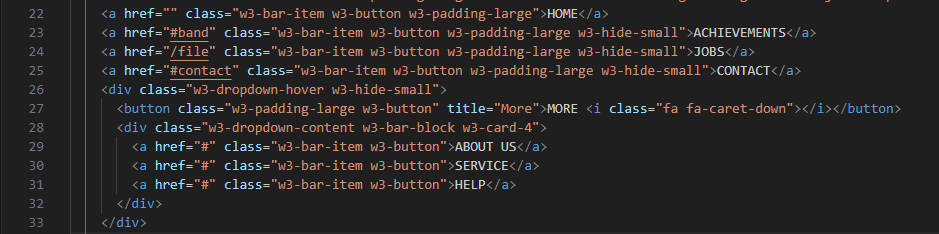
\includegraphics[width = 14 cm]{website.png}
		\caption{Home page NAV bar}
		\label{ab}	\end{center}
\end{figure}
%
%\bigskip\bigskip\bigskip\bigskip\bigskip
\section{Back-using python flask framework}
The following Python code will be divided into seven major steps. Lines of comments are included to provide a brief explanation and guide you through the coding process.
\subsubsection{Step #1: PDF file opening, reading and text extraction} 
\begin{figure}[h]
	\begin{center}
		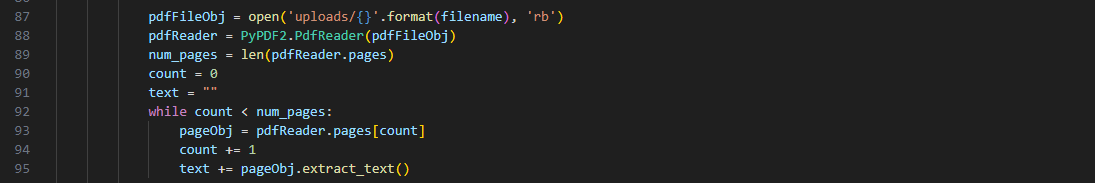
\includegraphics[width = 14 cm]{step1.png}
		\caption{PDF extraction}
		\label{ab}	\end{center}
\end{figure}

\subsubsection{Step #2: Text cleaning} 
\begin{figure}[h]
	\begin{center}
		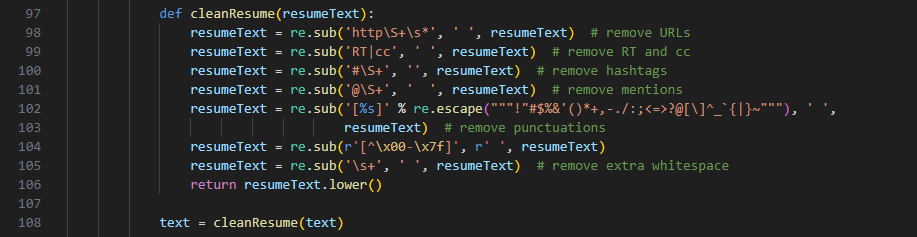
\includegraphics[width = 14 cm]{step2.png}
		\caption{Text cleaning}
		\label{ab}	\end{center}
\end{figure}

\subsubsection{Step #3: Extracting Email id from PDF} 
\begin{figure}[h]
	\begin{center}
		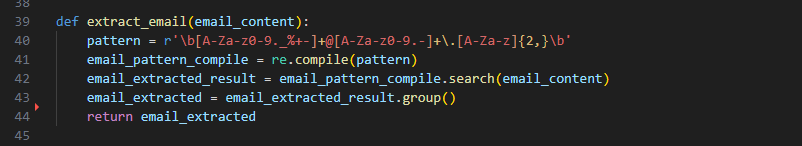
\includegraphics[width = 14 cm]{step3.png}
		\caption{Extracting Email}
		\label{ab}	\end{center}
\end{figure}

\subsubsection{Step #4: Dictionary with key terms by area setup} 
\begin{figure}[h]
	\begin{center}
		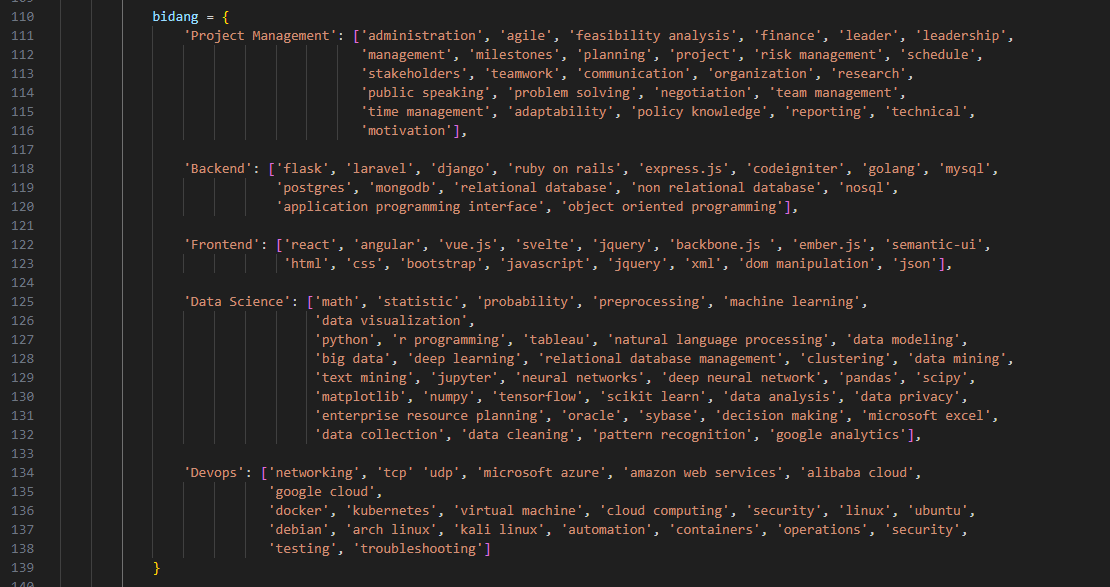
\includegraphics[width = 12 cm]{Dictionary.png}
		\caption{Dictionary}
		\label{ab}	\end{center}
\end{figure}

\subsubsection{Step #5: Scores calculation per area} 
\begin{figure}[h]
	\begin{center}
		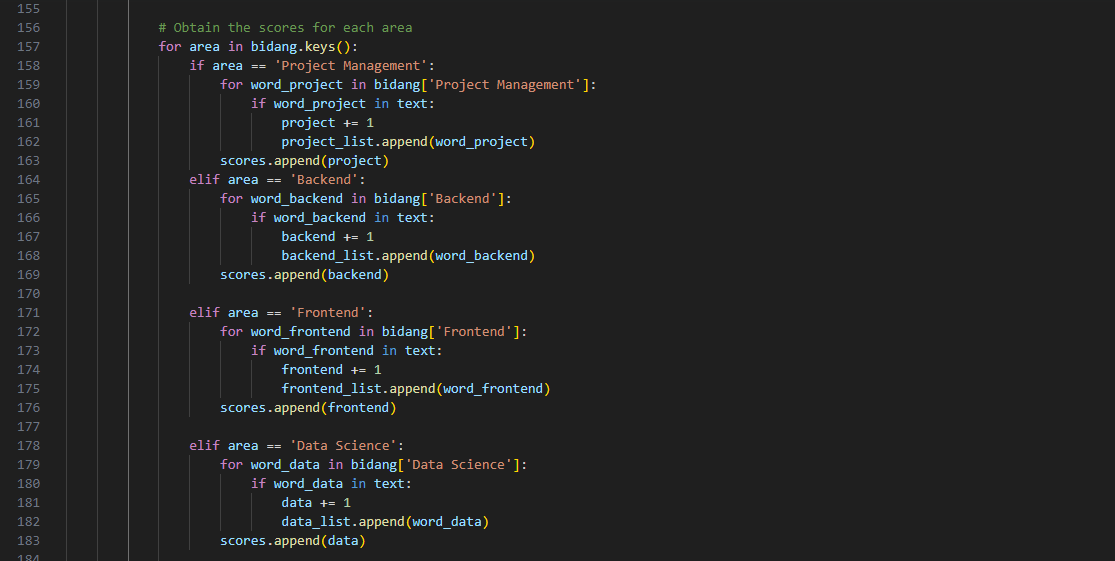
\includegraphics[width = 12 cm]{Scores.png}
		\caption{Score calculation}
		\label{ab}	\end{center}
\end{figure}

\subsubsection{ Step #6: Sorted data frame for final scores creation and Pie chart creation} 
\begin{figure}[h]
	\begin{center}
		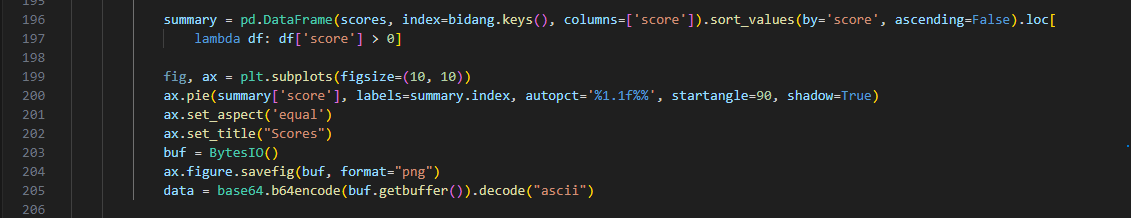
\includegraphics[width = 14 cm]{dataframe_piechart.png}
		\caption{Sorted data frame and pie chart creation}
		\label{ab}	\end{center}
\end{figure}
\section{Mail Sending}
\subsubsection{Sending mail with condition}
\begin{figure}[h]
	\begin{center}
		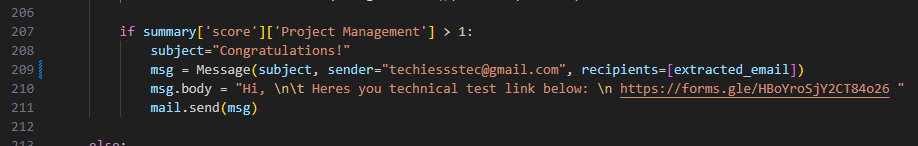
\includegraphics[width = 14 cm]{Email.png}
		\caption{Email extracted from pdf and sending with satisfying the condition}
		\label{ab}	\end{center}
\end{figure}


\chapter{IMPLEMENTATION AND PERFORMANCE EVALUATION}



%When implementing MIRNet for dark image enhancement, the following steps are typically involved:
%\begin{enumerate}
 %\item  Dataset Preparation: A dataset of low-light or dark images is collected for training the MIRNet model. The dataset should include pairs of input dark images and corresponding ground truth images that are properly exposed or enhanced.

 %\item  Network Architecture: The MIRNet architecture consists of multiple convolutional layers and residual blocks. It utilizes a multi-scale approach to capture both global and local image details. The network is designed to learn the mapping function between the low-light input images and their enhanced versions.

 %\item  Training: The MIRNet model is trained using the collected dataset. The training process involves optimizing the model's parameters to minimize the difference between the enhanced output images and the corresponding ground truth images. This is typically done by minimizing a loss function such as mean squared error (MSE) or perceptual loss.

 %\item  Data Augmentation: To improve the model's robustness and generalization, data augmentation techniques like random cropping, rotation, flipping, and adding noise may be applied to the training dataset. These augmentations help the model learn to handle different lighting conditions and variations in real-world images.

 %\item  Post-processing: After the MIRNet model produces an enhanced output image, post-processing techniques can be applied to further refine the results. These techniques may include denoising filters, histogram equalization, or tone mapping to improve contrast and color balance.

 %\item  Deployment: Once the MIRNet model is trained and tested, it can be deployed to enhance dark images in real-time or in batch processing. The model takes a low-light image as input and produces an enhanced image as output, effectively improving its brightness, reducing noise, and enhancing its visual quality.
%\end{enumerate}


%\begin{figure}[h]
%	\begin{center}
%		\includegraphics[width =13 cm]{UI.jpeg}
%		\caption{HOME PAGE}
%		\label{ab}
%	\end{center}
%\end{figure}

%\begin{figure}[h]
%	\begin{center}
%		\includegraphics[width =13 cm]{OP.png}
%		\caption{SAMPLE OUTPUT USING THIS PROJECT}
%		\label{ab}
%	\end{center}
%\end{figure}
%\bigskip\bigskip\bigskip\bigskip
\section{Web Page Home}
\begin{figure}[h]
 \begin{center}
		
\includegraphics[width = 8 cm]{home.png}
		\caption{Home page of Company website}
		\label{ab}	\end{center}
\end{figure}
\begin{figure}[h]
 \begin{center}
		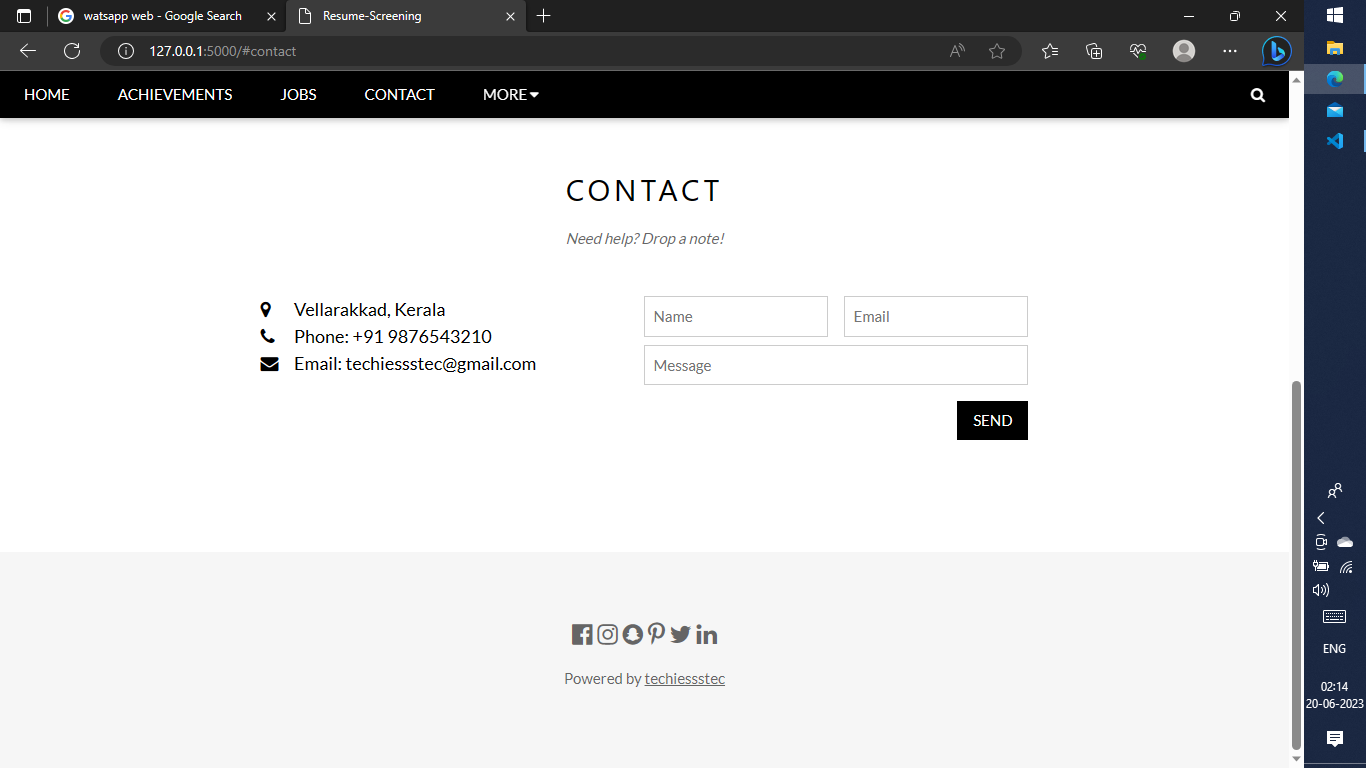
\includegraphics[width = 8 cm]{contact.png}
		\caption{Contact info in the website}
		\label{ab}	\end{center}
\end{figure}

\section{Resume uploading}
\begin{figure}[h]
 \begin{center}
		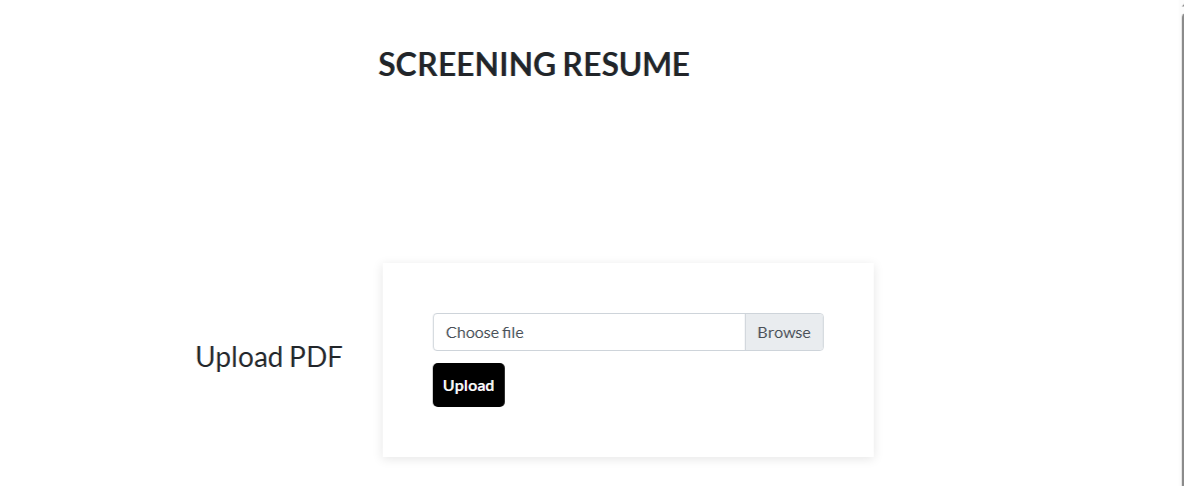
\includegraphics[width = 10 cm]{uploading.png}
		\caption{Resume uploading page}
		\label{ab}	\end{center}
\end{figure}

\section{Performance graph - Pie Chart}
\begin{figure}[h]
 \begin{center}
		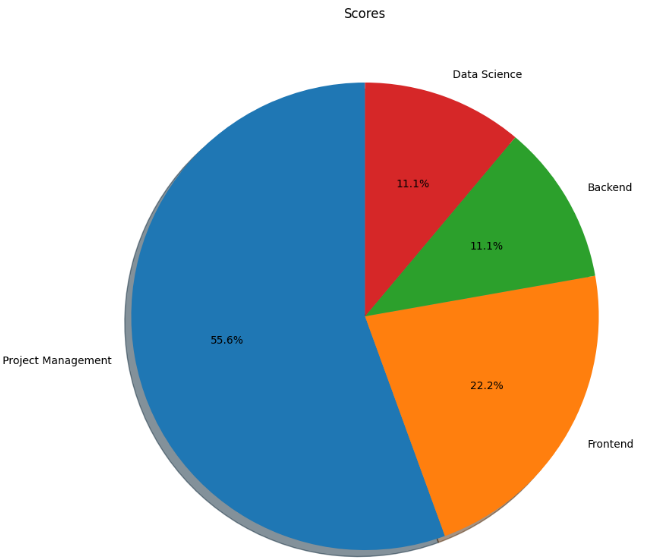
\includegraphics[width = 10 cm]{piechart_img.png}
		\caption{Pie Chart}
		\label{ab}	\end{center}
\end{figure}

%Dark image enhancement is an important task in computer vision, aiming to improve the visibility and quality of images captured in low-light conditions. MIRNet (Multi-scale Residual Network) is a deep learning-based method that has shown promising results in dark image enhancement. Here's a comparative study between MIRNet and some other popular methods for dark image enhancement:

%\subsection{Retinex-based Methods}
%Retinex-based methods aim to enhance the image by separating the reflectance and illumination components. Traditional Retinex algorithms, such as Single-scale Retinex (SSR) and Multi-scale Retinex (MSR), have been widely used. These methods suffer from issues like color distortion, halo artifacts, and over-enhancement in some cases.

%Comparative Study:
%MIRNet improves upon Retinex-based methods by leveraging deep learning techniques to learn more robust and effective features. It outperforms traditional Retinex algorithms by reducing color distortion, halo artifacts, and preserving more details in the enhanced images.

%\subsection{Histogram Equalization} 
%Histogram equalization is a simple and widely used method for enhancing the contrast of an image. It redistributes the pixel intensities to span the entire dynamic range. However, it may lead to over-enhancement and produce unnatural-looking images.

%\subsection{Deep Learning-based Methods}
%Various deep learning-based methods have been proposed for dark image enhancement, including CNN-based models like EnhanceNet and LIME, and GAN-based models like Pix2Pix and CycleGAN.

%Comparative Study:
%MIRNet demonstrates competitive performance compared to these deep learning-based methods. It benefits from the multi-scale residual architecture, which captures both global and local information effectively. MIRNet achieves better image enhancement by leveraging a hierarchical fusion strategy and reducing artifacts commonly present in GAN-based methods.

%\subsection{ Low-light Image Enhancement Network (LIME)}
%LIME is a deep learning-based method specifically designed for low-light image enhancement. It employs an encoder-decoder architecture with skip connections to enhance the details and contrast in dark images.

%Comparative Study:
%MIRNet outperforms LIME by utilizing multi-scale residual blocks that effectively capture hierarchical features. MIRNet provides superior results by preserving more details, reducing noise, and enhancing the overall brightness and contrast.

%It's worth noting that the performance of different methods can vary depending on the specific dataset and evaluation metrics used. While this comparative study provides a general overview, it's recommended to consult the original research papers for more detailed insights and performance comparisons on specific benchmark datasets.
\newpage
\section{Mail Execution Checking}
\begin{figure}[h]
 \begin{center}
		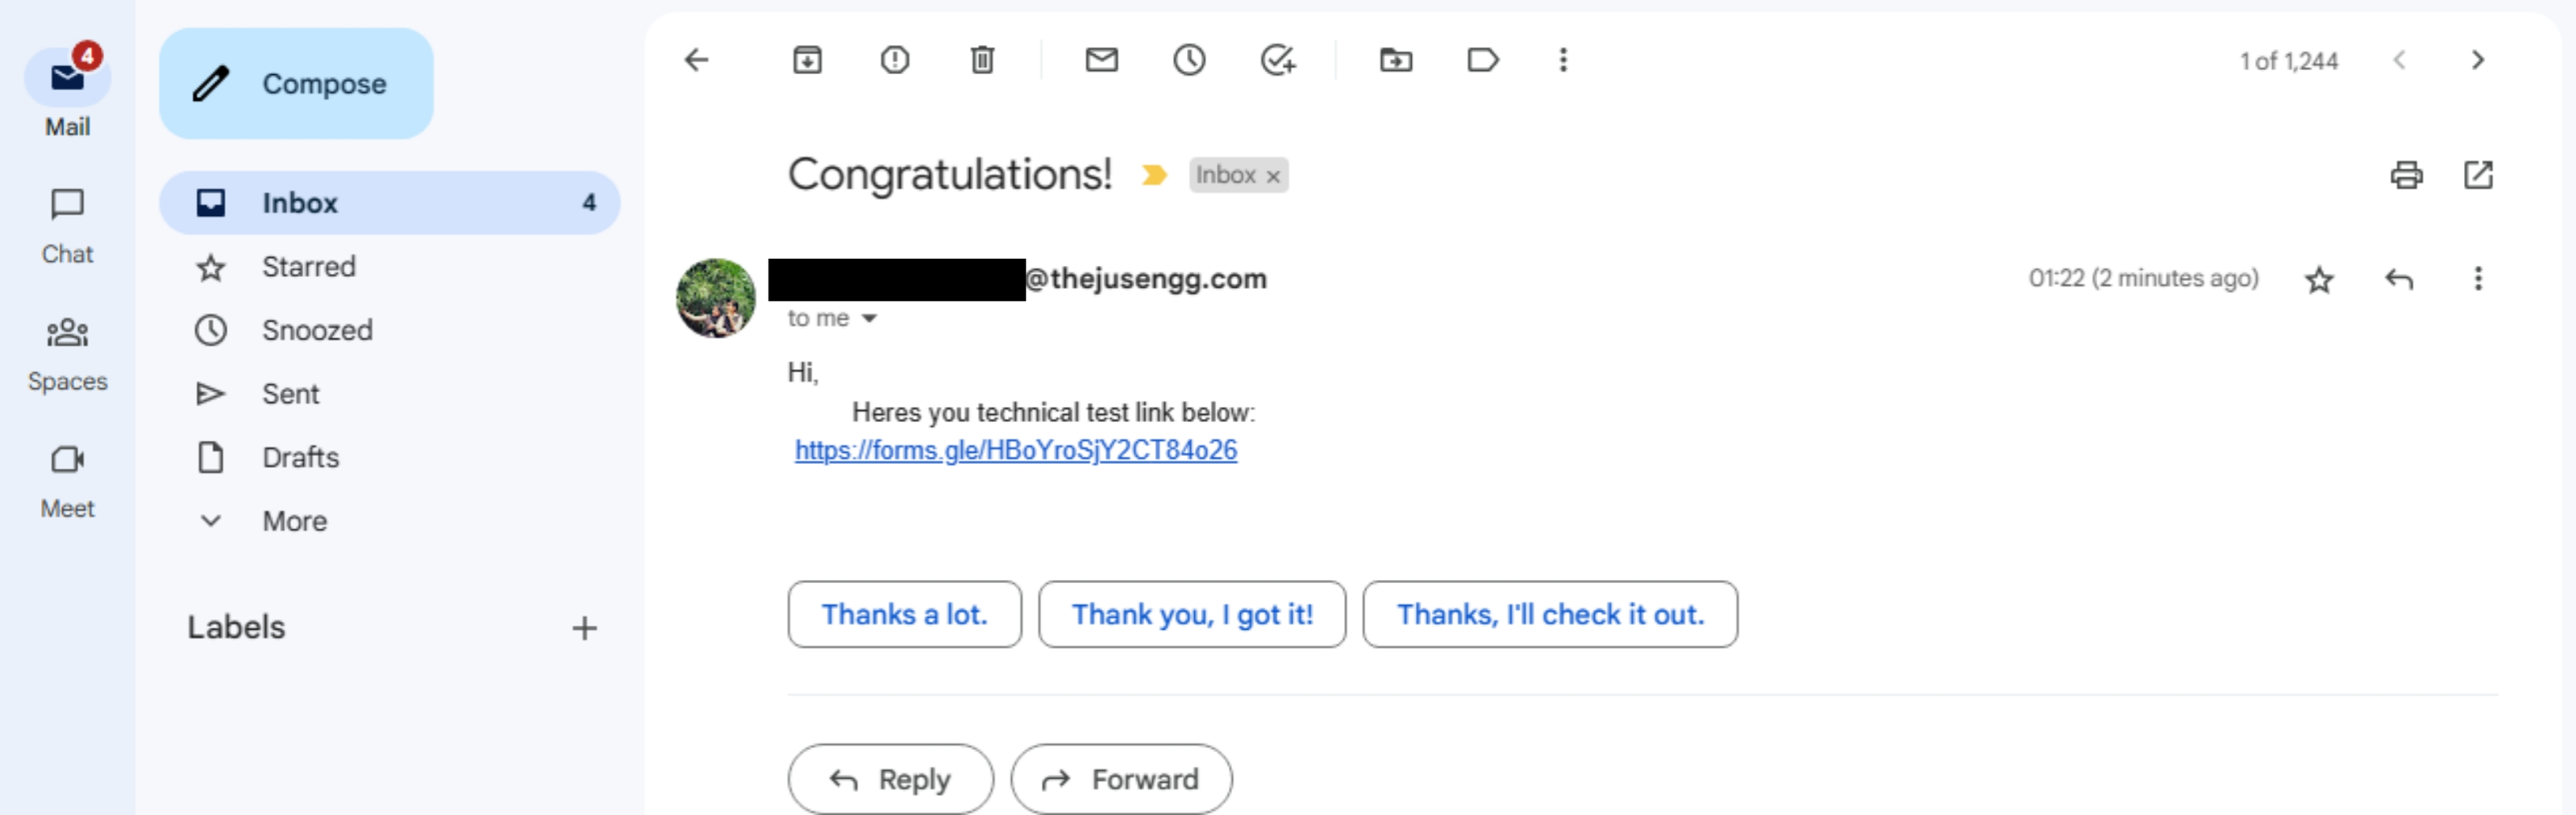
\includegraphics[width = 14 cm]{Emailsend.jpg}
		\caption{Email extracted from pdf and sending with satisfying the condition}
		\label{ab}	\end{center}
\end{figure}
%\begin{figure}[h]
%	\begin{center}
	    
	
%		\includegraphics[width =10cm]{PSNR.png}
%		\caption{TRAIN AND VALIDATION LOSSES OVER EPOCHS}
%		\label{ab}
%	\end{center}
%\end{figure}
%\begin{figure}[h]
%	\begin{center}
	    
	
%		\includegraphics[width =10 cm]{PSNR2.png}
%		\caption{TRAIN AND VALIDATION PSNR OVER EPOCHS}
%		\label{ab}
%	\end{center}
%\end{figure}



\chapter{ADVANTAGES AND DISADVANTAGES}
\section{Advantages}
\begin{enumerate}

\item  Easy uploading to multiple job-search sites and social media so that candidates far and wide will know you are hiring:\\
Social media should not be underestimated in the hiring process.

\item Scientific and psychometric assessments to ensure only quality candidates make the cut:\\
Most resume screening software only looks for keywords: candidate screening software examines not just whether they can do the job, but how they will do it and apply their values, personal traits, and behaviours to their duties.

\item Customized interviews:\\
A staff accountant needs different interview questions than an administrative assistant to determine if they’re truly a good fit, and each company offers a different product or service so interviews are not one size fits all. As an added bonus, you or your hiring managers don’t need to spend time making up questions to ask.

\item Eliminate costly screening calls:\\
Taking notes on just one candidate can take up to two hours of your or your employees’ valuable time. A streamlined screening solution will make this process much easier.

\item Seamlessly integrate with in-house talent management solutions"\\
The days of cumbersome employee files and performance evaluations are over, and candidate screening software can be a gateway for improving your existing talent management.

\item Cut down on time sitting through interviews:\\
Candidate screening software sorts through the available talent ahead of time and ensuring they have the necessary experience and skills for the job, you won’t waste time interviewing unsuitable candidates and can shorten interviews with the best candidates.

\item Decrease turnover rates:\\
Candidates who have not just the right skills and experience but also the personal values, traits, and methods that gel with your company’s culture will be less likely to seek opportunities elsewhere than candidates who are skilled but simply go through the motions at your workplace.

\item Make more confident hiring decisions:\\
Interviews and resumes aren’t enough to really determine who is the best fit for your business. Using a scientific-based approach to screen candidates’ problem-solving and interpersonal skills, values, and traits will lend you more confidence to making the right hiring decisions.

\item Save time sorting through resumes:\\
You’ll get inundated with job seekers regardless of the position, and sorting through resumes can take days.

\item Convenient dashboard for all communications and relevant documents:\\
Searching through email and files to find a candidate’s resume, application, cover letter, and other documents can create a time-consuming mess, candidate sorting software helps keep all communications and documents received from candidates in one convenient location.
\end{enumerate}

\section{Disadvantages}
\begin{enumerate}
\item Keywords are Created Based on A Previous Job Description:\\
Cultivating the best match between a company and a prospective hire is not based on job descriptions and criteria for the last person who worked the job. Companies should be looking for someone to step into the position that can make it better. Resume screening programs cannot find that person based on keywords constructed from previous job descriptions.

\item The Application Process is Off-Putting:\\
When you’re facing a shortage of qualified candidates that will add value to your company, is your first thought, “Let me make the application process as tedious and repellant as possible?” Resume screeners are built on a foundation of faulty logic. Resume screening was created to weed out unsuitable candidates instead of recruiting suitable ones.

\item Applicants Can Work the System:\\
A brief Google search pulls up over 24,000 search results for how to beat a resume screener. Applicants have caught onto the process of screening based on keywords and will stuff their resumes full of them to move onto the next stage of the hiring process. This means that the applicants who are usually approved by resume screeners know how to use keywords appropriately, but that does not necessarily make them the best person for the position. A candidate with better skills might be left in the slush pile.

\end{enumerate}


\chapter{CONCLUSION AND FUTURE ENHANCEMENTS}
\section{Conclusion}

Presently, we have seen the technology reaching new heights than ever ahead. But each association has a different way of working but for this they need people who have a specific skill set. Selection of the candidate is done on the base of seeing the skill set mentioned in the person's capsule who is applying at the organization. 
\newline
\par Technology is making the job search process easier and harder. Larger pools of applicants and limited opportunities force candidates to write outstanding resumes capable of defeating the “bots”. It is highly recommended for candidates to optimize their resumes keywords to represent their soft and hard skills and avoid including buzzwords. It is crucial for candidates to know how resume screening systems work to beat them and get their resumes to be viewed by a talent acquisition professional.
\newline
\par Resume screening is one of the most critical step in the recruitment cycle. It makes screening easier for the recruiters. Generally, resumes are sorted manually but, going through the resumes of these people manually is extremely time- consuming and lower effective as there are chances of human intervention error. Hence, the project designs a software which will sort all the resumes according to the demand of the company and reduce the working time for further recruitment process.

\par The algorithm will work in such a way that when a resume is to be scanned it will search only for the words according to the demand by the company and sort it accordingly. The required resume is shortlisted and the rest are auto rejected by the model. This will give high effectiveness compared to the manual sorting and give produce good results. This will lots of time and work of recruiters.


\section{Future Enhancements}
A well-structured resume clearly highlights your most attractive skills and experience to potential employers. This allows them to move forward with the best candidate. It's important to make sure your most recent skills and experiences are reflected in your resume for this reason.
\newline
\par Future work for this system  includes mining social networking data  (e.g. Facebook, LinkedIn,  GitHub profiles) of  the candidates and utilising  this social behaviour information in combination with resume content to make even  more  improved  recommendations.  
\newline 
\par Another  possibility  is  using  a collaborative  filtering  based  approach  that  can  match  the  current applicant  with  a  job  according  to  how  well  other  similar  candidates (neighbours) are rated for it. Another scope of future work lies in the use of Latent Semantic Analysis (Berry, M., 2001) in the calculation of semantic similarity between the documents and then comparing it with the results of the term frequency based similarity approach.
\newline
\par Scoring can be done based on weights given to each parameters. Higher weights can be given to more relevant parameters. The relevancy of the parameters can be measured using past recruitment trends.
\newline
\par Personality analysis can be done of the shortlisted candidates using social media information provided in the resumes. this analysis will help to judge whether the candidate's personality as per his/her social life matches the job requirements.
\newline
\par The future versions of this application will include more types of resumes or templates, and it will accept input in any extended format  such as .pdf or .docx, so that the object detection range can be expanded. 
Additionally, we work to manage job descriptions that require more evaluation criteria, such as soft skills or qualifications relevant to a certain industry. More complex evaluation criteria may be added in the future to increase the accuracy of candidate matching.
\newline
\par These potential future enhancements can contribute to further advancements in resume screening. By addressing specific challenges and incorporating user feedback, the model can continue to evolve and deliver more accurate, and adaptable results in the future.

























%
%
%
% ***   Creating Bibliography   ***
%
% Do not delete the following two lines
%
\clearpage
\addcontentsline{toc}{chapter}{\quad BIBLIOGRAPHY}
%
%   The markups for creating the bibliography 
%   begins here. Do not change the two lines 
%   "\begin{thebibliography}{99}" and 
%   "\end{thebibliography}".
%   One sample bibliography item is included. 
%   Each new item is to be preceded by
%   "\bibitem{}".
%   Add additional items if there are any.
%   Bibliography styles:
%   Titles of books   : Italics  {use {\em Title} )
%   URLs of websites  : Type-writer (use {\tt Title} )
%   Titles of papers  : In double quotes (use ``Title")
%
\begin{thebibliography}{99}
%
\bibitem{ref1}
https://github.com/aarshps/photo-gallery-python-flask 

\bibitem{ref2}
https://phoenixnap.com/kb/install-flask
  
\bibitem{ref3}
https://testdriven.io/courses/learn-flask/intro/

\bibitem{ref4}
https://www.digitalocean.com/community/tutorials/how-to-make-a-web-application-using-flask-in-python-3

\bibitem{ref5}
 https://www.digitalocean.com/community/tutorials/how-to-make-a-web-application-using-flask-in-python-3

\bibitem{ref6}
https://www.digitalocean.com/community/tutorials/how-to-create-your-first-web-application-using-flask-and-python-3

\bibitem{ref7}
https://pemagrg.medium.com/build-a-web-app-using-pythons-flask-for-beginners-f28315256893

\bibitem{ref8}
https://www.digitalocean.com/community/tutorials/how-to-use-web-forms-in-a-flask-application

\bibitem{ref9}
 https://www.geeksforgeeks.org/how-to-upload-file-in-python-flask/

\bibitem{ref10}
https://towardsdatascience.com/resume-screening-with-python-1dea360be49b

\bibitem{ref11}
https://youtu.be/ejLGwHiyqGU

\bibitem{ref12}
https://www.w3schools.com/html/html-form-attributes-form.asp

\bibitem{ref13}
https://youtu.be/1oOefRD8jek




%
\end{thebibliography}
%
%   ***   Creating Index   ***
%
%   To add a particular word, say abcxyz, to index write 
%   the command \index{abcxyz} near the word where it 
%   first appears in the text. Include all technical 
%   sounding words in the index. 
%   Do not delete the following three lines.
%
%\clearpage
%\addcontentsline{toc}{chapter}{\quad INDEX}
%\printindex
%
\clearpage


%%%%%%%%%%%%%%%%%%%%%%%%%%%%%%%%%%%%%
%%%%%%%%%%%%%%%%%%%%%%%%%%%%%%%%%%%%%
%%                      
%%                      For Adding PDF (Data Sheets) for the Appendix
%%
%%%%%%%%%%%%%%%%%%%%%%%%%%%%%%%%%%%%%
%%%%%%%%%%%%%%%%%%%%%%%%%%%%%%%%%%%%%



%%%%%%%%%%%%%%%%%%%%%%%%%%%%%%%%%%%%%
%%%%%%%%%%%%%%%%%%%%%%%%%%%%%%%%%%%%%
%%%%%%%%%%%%%%%%%%%%%%%%%%%%%%%%%%%%%
%%%%%%%%%%%%%%%%%%%%%%%%%%%%%%%%%%%%%




%   Printing the last page
%
\end{spacing}
\newpage
\thispagestyle{empty}
\vspace*{\fill}
\begin{flushright}

\includegraphics[width=2.5 cm]{thejus.png}\\[.2 cm]
{\Large \bf \rm  Department of \vdept\ }\\
{\large \rm Thejus Engineering College\\
Vellarakkad, Thrissur - 680 584\\
({\tt http://www.thejusengg.ac.in})}
\end{flushright}

%
%
%
%   ***   The end   ***
%
%
\end{document}


%%%%%%	Any Problems Contact me  @  Comments at Youtube Channel 

%   https://www.youtube.com/c/arunxaviertech
%
%  arunxeee.blogspot.com 
%%%%%			
%%%%%%%%%%%%%%%%
%%%%
%%%%
%%%%%%%%%%%
%%
%
